\documentclass[11pt]{article}
\usepackage[letterpaper,margin=1in]{geometry}
\usepackage{fontspec}
\usepackage{polyglossia}
\setdefaultlanguage{english}
\PolyglossiaSetup{english}{hyphenmins={2,3}}
\usepackage{newunicodechar}
\newunicodechar{α}{\ensuremath{\alpha}}
\newunicodechar{κ}{\ensuremath{\kappa}}
\newunicodechar{≥}{\ensuremath{\geq}}
\newunicodechar{≤}{\ensuremath{\leq}}
\newunicodechar{−}{\ensuremath{-}}
\newunicodechar{×}{\ensuremath{\times}}
\newunicodechar{→}{\ensuremath{\rightarrow}}
\newunicodechar{≈}{\ensuremath{\approx}}
\newunicodechar{±}{\ensuremath{\pm}}
\usepackage{graphicx}
\usepackage{booktabs,longtable,array,calc,tabularx,makecell}
\renewcommand{\cellalign}{lb}\setcellgapes{1pt}
\usepackage{caption}
\captionsetup{font=small,labelfont=bf}
\captionsetup[table]{skip=4pt}
\usepackage{xcolor}
\definecolor{doired}{RGB}{140,20,20}
\usepackage[hidelinks=false,colorlinks=true,linkcolor=black,citecolor=black,urlcolor=doired,pdfauthor={Marin T. Kael},pdftitle={Report 04 · Book Launch and AI Citation},pdfcreator={},pdfproducer={}]{hyperref}
\usepackage{url}
\setlength{\parindent}{1.5em}
\newcounter{none}
\providecommand{\pandocbounded}[1]{#1}
\makeatletter\def\fps@figure{htbp}\makeatother
\usepackage[section]{placeins}
\usepackage{needspace}
\providecommand{\tightlist}{\setlength{\itemsep}{0pt}\setlength{\parskip}{0pt}}
\renewcommand{\tablename}{Table}
\renewcommand{\figurename}{Figure}
\setlength{\emergencystretch}{3.5em}
\renewcommand{\floatpagefraction}{0.8}
% Schlusszeile: letzte zwei Wörter gekoppelt, letztes Wort ungetrennt (build_paper.py, last_two)
\finalhyphendemerits=0
% Satzregeln (08.11.2026): keine einzelne Absatzzeile oben/unten auf einer Seite, keine Trennung über den Seitenumbruch,
% keine zweibuchstabigen Trennreste; Gleitseiten oben bündig; Tabellenbeschriftungen im Flattersatz (keine gesperrten Zeilen)
\widowpenalty=10000 \clubpenalty=10000 \displaywidowpenalty=10000
\brokenpenalty=10000
\makeatletter\setlength{\@fptop}{0pt}\setlength{\@fpsep}{14pt}\setlength{\@fpbot}{0pt plus 1fil}\makeatother
\captionsetup[table]{justification=raggedright,singlelinecheck=false}
% Aufzählungen mit knappem Abstand davor und danach (sonst passte auf Seite 2 der erste Listenpunkt nicht mehr, Lücke, 08.11.2026)
\makeatletter\g@addto@macro\@listi{\setlength{\topsep}{3pt plus 1pt minus 1pt}\setlength{\partopsep}{0pt}}\let\@listI\@listi\@listi\makeatother
\begin{document}
% Namen ohne Trennung: Liste NO_HYPH in build_paper.py, dort auch die Abbruchprüfung am PDF-Text.
\hyphenation{CUSUM OpenAI Gemini Claude Sonnet Opus Haiku Google Pauline Kael Marin Zenodo ORCID GitHub}
\begin{center}
{\LARGE\bfseries Report 04 · Book Launch and AI Citation\par}
\vspace{4pt}
{\large Does the release of “Das vierte Feld” change how AI answer engines cite its author? Before-after analysis of pre-registration Q7, baseline 8~September to 7~October, effect window 8~October to 7~November~2026\par}
\vspace{14pt}
{\large\bfseries Marin T. Kael\par}
\vspace{2pt}
Independent researcher -- AI Citation Field Lab\par
\texttt{marin@marin-t-kael.de}\quad ORCID: 0009-0006-2105-8190\par
\vspace{12pt}
{\large November 2026 \quad$\bullet$\quad DOI \href{https://doi.org/10.5281/zenodo.24063460}{10.5281/zenodo.24063460}\par}
\end{center}
\vspace{6pt}
\begin{abstract}
This report tests the pre-registered hypothesis that the retail availability of the first volume on 8~October~2026 changes how AI answer engines with web search cite the author, earlier in the Direct channel than in the Recommendation channel. The primary analysis covers OpenAI with web search and Gemini with Google web search on the anchor days of the three-day grid; the baseline runs from 8~September to 7~October, the effect window from 8~October to 7~November~2026.

In the baseline the headline averaged 22.45~percent across both providers (OpenAI 23.96 on 6~anchor days, Gemini 20.94 on 10~anchor days), and in the effect window, again as the mean of the two provider means, 25.83~percent (OpenAI 25.62 on 10~anchor days, Gemini 26.04 on 5~anchor days). From 24~October Gemini is missing because its credit was used up. Without drift removal the difference is thus +3.38~percentage~points; drift-adjusted, as pre-registered, it is +1.38~percentage~points (95 \% interval −3.59~to 6.68). The interval includes zero; the null hypothesis is not~\mbox{rejected.}

No channel interval excludes zero either: Direct −0.19 (−15.51~to 15.53), Saga knowledge +0.37 (−20.94~to 22.34), Recommendation +2.27 (−3.02~to 8.11), of which GR1~to~GR6 +3.79 (−5.42~to 13.48). Neither Direct nor Recommendation shows a first deviation up to 5~November; the order hypothesis receives no support, also with the pre-registered Recommendation channel GR1~to~GR6. Only the headline and the hit rate across all questions raise an upward alarm, both on 5~November, a day measured by OpenAI~\mbox{alone.}

In the baseline measurement on 7~October Claude on claude.ai stood at 8.34~percent as the mean of the three models (Direct 44.44, Saga knowledge and Recommendation 0.00) and from 4.86~to 9.03~percent on the 10~anchor days; no recommendation named the author on any day. These values are~\mbox{descriptive.}

Against the sensitivity baseline without early availability (8 to 29~September) the headline difference is +0.74 (−5.08~to 8.22); with the scoring rules of 2~November in both windows it is +2.77 (−2.37~to 8.28), with empty answers treated as gaps +1.70 (−3.27~to 6.96) and without amendment~4 +0.96 (−4.15~to 6.36). All of these lead to the same decision. If empty answers are treated as failed measurements, Gemini keeps one effect day and no interval can be computed. An extension of the effect window to anchor day 8~November, on which Gemini is measured again, is not pre-registered and gives +2.32 (−2.74~to 7.95); the decision rests on the pre-registered main analysis alone. OpenAI is fully measured on all 10~anchor days of the effect window, Gemini on~\mbox{5.}

\end{abstract}
% Seite 1 nur Titel und Zusammenfassung; Abschnitt 1 beginnt auf Seite 2 (Hinweis 08.11.2026: Überschrift mit zwei Zeilen am Seitenende)
\clearpage
\Needspace{6\baselineskip}\section{Research question and pre-registration}

The programme studies when and how AI answer engines find and cite a new author. Until early October~2026 almost all evidence about the author and his work was self-published. The release of the first volume creates, for the first time, evidence that third parties maintain and publish in machine-readable form: retailer catalogues, library metadata, ISBN~\mbox{registers.}

The first version of pre-registration Q7 was recorded in the data-gap register on 5~September~2026, at that time for a release on 22~September (entry~12). On 15~September the release was moved publicly to 8~October; the re-dated version was recorded on 23~September (entry~18), before the event. The pre-registration file has been in the repository since 7~October~2026; a dated note of 8~November~2026 records the registration dates there and leaves the original statements of the file unchanged. Hypothesis: search-grounded models retrieve the new third-party evidence, so that the hit rate in the Direct channel (questions D1~to~D3) rises earlier than in the Recommendation channel (questions GR1~to~GR6), because recommendations additionally need reception signals. Null hypothesis: no difference between the measurement windows. Metric: the headline per anchor day and the three channels Direct, Saga knowledge and Recommendation. Analysis: before-after comparison with the baseline drift removed, so that a running trend is not read as an effect. The 16 fixed questions and the three-day grid remain~\mbox{unchanged.}

On 7~October~2026, one day before the event, the pre-registration was amended (version~1.1, entry~36). The amendment was prompted by measurement changes that touch the commitment not to adjust the provider panel. They are justified by measurement problems (Claude entries from 16~September to 6~October and entry~34); interim results played no part in the amendment. The amendment has four~\mbox{points:}

\begin{enumerate}
\def\labelenumi{\arabic{enumi}.}
\tightlist
\item
  The primary analysis uses only the two providers whose panel has been unchanged since 19~August: OpenAI with web search and Gemini. The headline is the simple mean of both providers per anchor day, plus the three channels. The baseline covers 10~anchor days for Gemini and 6 for OpenAI, because the OpenAI measurement failed from 18 to 27~September (entry~17). Hypothesis, null hypothesis and analysis are~\mbox{unchanged.}
\item
  Claude is analysed only as a secondary, descriptive series. From 7~October the programme measures with the newest Opus model on claude.ai in an incognito chat with web search (entry~34). The earlier series of three model tiers is not comparable. The only baseline of the new configuration is one measurement on 7~October outside the grid, followed by anchor days from 9~October. There is no significance judgement for~\mbox{Claude.}
\item
  Paperback and hardcover could be ordered from 30~September; the official release and the ebook followed on 8~October. A sensitivity baseline from 8 to 29~September without early availability is therefore reported in~\mbox{addition.}
\item
  The scoring correction of 7~October affects Claude rows only (entry~32), and restricting the trend display to anchor days affects the display only; neither touches the primary~\mbox{analysis.}
\end{enumerate}

Point 4 is corrected by a second amendment, fixed on the same day before the event and without knowledge of effect data (amendment~2, version~1.2, entry~38). It has three~\mbox{parts:}

\begin{enumerate}
\def\labelenumi{\arabic{enumi}.}
\tightlist
\item
  Correction to point 4: a further correction of the scoring scheme also affects OpenAI and Gemini (entry~37). The scheme still listed the old release date of 22~September as a core fact; from 7~October the date counts whether an answer names 22~September or 8~October. Since 15~September only answers whose stored 500-character excerpt itself proves the core facts were re-scored: 8~answers from two to three points. Because the baseline could only be partly re-scored while the effect window is scored fully under the new rule, the point-based Direct channel may be biased upwards. The baseline of this report includes these 8 and further re-scorings of the same day (section~2).
\item
  Robustness metric: the hit rate, the share of answers that name the author correctly (score above zero), per provider and channel. It does not depend on the threshold between partial and full citation. A Direct-channel effect was to be reported only if it appears in points and in the hit rate; this rule is replaced by amendment~3.
\item
  Analysis details: drift, effect estimate and first deviation as in section~3; the last anchor day of the effect window is 5~November.
\end{enumerate}

A third amendment, also fixed on 7~October before any effect data (amendment~3, version~1.3, entry~39), replaces the Direct rule of amendment~2. The reason is the ceiling of the Direct hit rate: in the baseline, on average across both providers, 92.2~percent of answers name the author correctly, so a rise can be at most 7.8~percentage~points, below the minimum detectable shift (section~4). In the Direct channel the hit rate now serves as a sign check only; in all other channels it remains a full robustness~\mbox{metric.}

A fourth amendment was fixed on 15~October~2026 during the effect window, after the anchor days 9, 12~and 15~October, and is disclosed as such (amendment~4, version~1.4, entry~50). It was prompted by an error in the scoring scheme found while reading answers: the scheme required the author name as an anchor, so an answer that named the book correctly without naming the author scored zero. Since then the book or series title also counts as an anchor when it is not already part of the question; the non-fiction book of the same title by another author remains a collision without points. The rule applies retroactively to all rows since 19~August. It changes two answers, both of 12~October on question L1: Gemini from zero to two points and Claude Opus from zero to two points (descriptive only). No baseline answer is affected, so the rule acts equally on baseline and effect window. Because amendment~4 changes a Gemini answer in the effect window, section~7 also reports the analysis without~\mbox{it.}

Besides the four amendments, four rules were registered on 7~October before the event. From 9~October Claude is measured with the newest model of each of the three families Opus, Sonnet and Haiku; the provider value is their mean (entry~41). The baseline measurement on 7~October also covers all three models, with Haiku still at Haiku 4.5 (entries~45~and 49). Answers that report an honest search non-result score zero instead of minus three (entry~42). A reference to the film critic Pauline Kael counts as a name collision with zero points; genuine statements about the author in the same answer are scored as usual (entry~43). These three rules leave the primary metric unchanged or act equally on baseline and effect window, entry~43 with one qualification. The scorer in its pre-registered version, that is before the rules of 2~November, implements the second part of entry~43 more narrowly: an answer that describes the author correctly and distinguishes him from Pauline Kael at the end is scored as a collision with zero points (fault 1 in entry~71). Before the event this concerned only one OpenAI or Gemini answer (Gemini, 6~September, question D1), which was re-scored according to the wording on 7~October. In the effect window it concerns 5 Claude answers to question D1, in the extension 6; here the main analysis follows the scorer, and OpenAI and Gemini are not affected (section~6). If OpenAI fails because its quota is exhausted, it is measured once more within 36 hours (entry~44). This rule acts only in the effect window, because the baseline contains no re-measurement; this is how 2~November enters for OpenAI (section~2). Three further rules followed inside the effect window. Since 1~November an empty answer counts as a failed measurement (entry~66), and from anchor day 5~November the question is then asked once more within the same run (entry~70); empty answers before 1~November enter with zero points. On 2~November four errors in the scoring rules were corrected, retroactively for the effect window; the measurement database carries the new rules from the measurement of 5~November (entry~71). The main analysis scores the effect window throughout under the pre-registered rules, with the scorer in its version before 2~November: it resets the ten retroactively changed answers, and the 64 scored answers of 5~November (16 from OpenAI, 48 from Claude) were re-scored on the full text under the pre-registered rules. Of these, one Claude answer differs, while the 16 OpenAI answers score the same under both rules; in total the main analysis resets eleven answers. A sensitivity analysis applies the new rules to the baseline as well (section~7). For Claude, web search is enabled but not forced; since 2~November each answer records whether a search took place (entry~72). After the effect window had closed, a catch-up rule for Gemini (entry~82) and the extension to anchor day 8~November, which is not pre-registered (entry~83, section~7), were added on 8~November. Section~8 summarises all deviations from the~\mbox{plan.}

\Needspace{6\baselineskip}\section{Data and windows}

The main analysis rests on two pulls from the measurement database. The baseline pull was frozen on 7~October~2026 with the cut-off 7~October, 23:59~UTC; the original files remain unchanged. Rows time-stamped before the cut-off that arrive later are stored separately as a supplement, changes to frozen rows until 8~October, 12:00~UTC, separately as a correction; later changes are only reported. The supplement holds the 48~answers of the Claude baseline measurement of 7~October (16 per model), the corrections 18 re-scored answers from OpenAI and Gemini (8 from entry~37, 9 from entry~42, one from entry~43) and 3 of the earlier Claude series. Of these, 3 Gemini answers fall on baseline anchor days (answers per day: 21~September 1, 3~October 2) and 3 on anchor days of the drift base (19~August, 25~August, 6~September). It contains 1,504 answer rows from OpenAI and Gemini between 19~August and 6~October, 1,008 answer rows of the earlier Claude series, the run times of the measurement runs and 35 entries of the data-gap register. The second pull was frozen on 8~November~2026, 04:11~UTC, with the cut-off 7~November, 23:59~UTC. It contains 1,824 answer rows from OpenAI and Gemini, 1,536 answer rows from Claude, 84 measurement runs and 78 register entries. Checked against this pull the baseline holdings are complete and unchanged: of 1,504 OpenAI and Gemini rows and 1,056 Claude rows, 0 are missing and 0 changed. For the extension, which is not pre-registered (section~7), a third pull was taken on 8~November~2026, 15:54~UTC, with the cut-off 8~November, 23:59~UTC, after all measurements of that day were in. It contains 1,856 answer rows from OpenAI and Gemini, 1,584 from Claude, 85 measurement runs and 82 register entries. Up to 7~November it matches the second pull (0~rows missing, 0 changed); new are the 32 answer rows from OpenAI and Gemini and the 48 from Claude of 8~November.

Each provider answers the same 16~questions: three name the author or the work (Direct, D1~to~D3), two ask about terms from the work (Saga knowledge, L1 and L2), ten name neither author nor work (Recommendation: two genre questions, two comparison questions, six recommendation questions GR1~to~GR6), and one asks about the research programme (R1). The channels follow the grouping of the measurement service; R1 enters the headline only. The pre-registration names questions GR1~to~GR6 as the Recommendation channel. Deviating from this, the Recommendation channel of the analysis comprises ten questions; this was fixed in the analysis code on 7~October, before the event, so that the channels follow the grouping of the measurement service, but it was not registered. The pre-registered channel GR1~to~GR6 is therefore reported throughout, including for the order hypothesis. Questions G1, G2, C1 and C2 score zero on every anchor day; the ten-question channel is therefore exactly 0.6 times the channel GR1~to~GR6 on every provider-day, in points and in the hit rate. Scoring is rule-based from minus three to plus~\mbox{three.}

\enlargethispage{\baselineskip}Only the anchor days of the three-day grid starting on 19~August~2026 are analysed. OpenAI and Gemini also measured on 30 intermediate days between 20~August and 4~October; these measurements are not used (entry~26).

\begin{table}[htbp]\centering\small
\caption*{\normalsize\textbf{Table~1:} Analysis windows and anchor days. The delayed-effect observation runs until 6~January~2027 and will be analysed afterwards as an addendum (section~\mbox{7).}}
\begin{tabularx}{\linewidth}{>{\raggedright\arraybackslash}X>{\raggedright\arraybackslash}Xlll}\toprule
Window & Period & \makecell[lb]{Anchor days} & \makecell[lb]{complete\\OpenAI} & \makecell[lb]{complete\\Gemini} \\\midrule
Drift base before baseline & 2026-08-19–09-07 & \mbox{7} & \mbox{7} & \mbox{7} \\
Baseline & 2026-09-08–10-07 & \mbox{10} & \mbox{6} & \mbox{10} \\
Sensitivity baseline & 2026-09-08–09-29 & \mbox{7} & \mbox{3} & \mbox{7} \\
Effect window & 2026-10-08–11-07 & \mbox{10} & \mbox{10} & \mbox{5} \\
Delayed-effect observation & 2026-11-08–2027-01-06 & \mbox{20} & \mbox{ongoing} & \mbox{ongoing} \\
Extension, not pre-registered & 2026-10-08–11-08 & \mbox{11} & \mbox{11} & \mbox{6} \\
\bottomrule\end{tabularx}\end{table}

The anchor days of the effect window are 9, 12, 15, 18, 21, 24, 27~and 30~October and 2~and 5~November. The release day itself is not an anchor day. The extension, which is not pre-registered (section~7), adds 8~November to the effect window; under the pre-registration it is the first anchor day of the delayed-effect observation. On the four baseline anchor days 18, 21, 24~and 27~September OpenAI returned error rows only; these days do not count for OpenAI, and a gap is not a zero. In the effect window OpenAI has 16 values on all 10~anchor days; on 2~November the interface first refused every question (quota exhausted), and the repeat measurement under the catch-up rule fell within the 36-hour limit (entries~44~and 68). Gemini refused every question on the anchor days 24~October, 27~October, 30~October, 2~November and 5~November because the credit of the measurement account was used up (entries~58, 61, 64, 67~and 74); no repeat measurement was made, and these days will not be re-measured later, because the catch-up rule for Gemini applies only from 8~November (entry~82). Gemini therefore contributes 5 effect anchor days, the headline is defined on 5~anchor days, and the remaining 5 are basis changes. Formally the per-provider estimate is unaffected, because each provider difference is computed against its own baseline; the Gemini difference, however, rests on the first half of the window only. There were no measurements on intermediate days in the effect~\mbox{window.}

\Needspace{6\baselineskip}\section{Methods}

For each anchor day, provider and question one answer counts, following the programme rule of 4~September~2026 (data-gap register, entry~11): an error row always loses; among the others, the answer whose time stamp is closest to the scheduled run time wins, ties go to the earlier one. The baseline pull contains no duplicate rows on anchor days. A provider's daily value is the score sum divided by the maximum (number of questions times three), as a percentage, separately for all 16~questions and for each channel. A provider-day counts only if all 16~questions have a value. The headline of an anchor day is the mean of OpenAI and Gemini and is defined only on days on which both measured; days with one provider are flagged as a change of basis and not~\mbox{averaged.}

The first version of the pre-registration fixes a before-after comparison with baseline drift removed but no details. These were fixed in the analysis code on 7~October~2026, before the event, and registered with amendment~2.

Drift. For each provider and channel a least-squares line is fitted over all anchor days from 19~August to the end of the baseline (OpenAI 13, Gemini 17~anchor days) and extended into the effect window. The longer period stabilises the slope, above all for OpenAI with only six baseline days. The level of the comparison remains the~\mbox{baseline.}

Difference. For each provider the drift-adjusted difference is the mean residual in the effect window minus the mean residual in the baseline, both against the same line. For the headline and each channel the mean of the two provider differences is reported; this uses all registered baseline days of both providers without a day-to-day change of basis. The unadjusted difference of means is reported~\mbox{alongside.}

Interval. The 95~percent interval comes from a bootstrap over anchor days with 10,000~draws and a fixed seed. Days are drawn with replacement, separately for the drift base before the baseline, the baseline and the effect window, and separately per provider; the line is refitted in every draw. The null hypothesis is rejected if the interval of the drift-adjusted difference excludes~\mbox{zero.}

Drift check. Whether the baseline shifted relative to the preceding period is checked with a tabular CUSUM chart with k = 0.5 and h = 5 standard deviations, as is standard in the programme, with the seven anchor days from 19~August to 6~September as~\mbox{reference.}

First deviation. For the order hypothesis a one-sided CUSUM is run per channel from the first anchor day of the effect window on the drift-adjusted residuals, standardised by their standard deviation in the baseline (k = 0.5, h = 5). The first anchor day with an alarm is the time of the first significant deviation. Because channels with few questions can be almost without variance in the baseline, the standard deviation is bounded below by half a score point of one provider measurement (headline 1.04, Direct 5.56, Saga knowledge 8.33, Recommendation 1.67, GR1~to~GR6 2.78~percentage~points). As a secondary criterion the first anchor day on which the residual exceeds the 95~percent prediction bound of the drift line is reported. The hypothesis counts as supported if the Direct channel raises an upward alarm within the window, before the Recommendation channel or without that channel alarming; if neither alarms, it receives no support. The verdict is formed with the ten-question Recommendation channel and repeated with the pre-registered channel GR1~to~GR6 (section~2).

Minimum detectable shift. The scatter around the drift line determines which shift is detectable with ten complete effect anchor days per provider at 80~percent power (two-sided, 5~percent): headline 4.68~percentage~points, Direct 14.84, Saga knowledge 20.12, Recommendation 4.61, GR1~to~GR6 alone 7.68. These values serve planning only; they were computed on 7~October, before the event, with the baseline corrected for entries~42~and 43, and treat the drift as known. Gemini has only 5 complete anchor days in the effect window (section~2). Taking into account the uncertainty of the drift line and the anchor days actually measured per provider, the minimum detectable shift is 7.32~percentage~points for the headline, 21.93 in the Direct channel, 31.12 for Saga knowledge, 7.96 for Recommendation and 13.52 for GR1~to~GR6, computed as 2.8 times the bootstrap standard deviation of the drift-adjusted estimate; these values are not~\mbox{pre-registered.}

Hit rate. As robustness metric (amendment~2) the share of answers scored above zero is computed per provider-day and channel and analysed with the same procedure: baseline, sensitivity baseline, drift line, drift-adjusted difference with bootstrap interval and CUSUM for the first deviation (lower bound of the standard deviation: half an answer of one provider measurement). In the Direct channel amendment~3 applies (entry~39): a point effect is reported if its interval excludes zero and the estimate of the hit-rate difference has the same sign; an estimate of zero does not count as the same sign. If the sign contradicts, the effect is classed as not robust. In the other channels an effect counts as robust if the intervals of the point difference and of the hit-rate difference both exclude zero and share the same sign. Minimum detectable shift of the hit rate: all questions 4.86~percentage~points, Direct 15.45, Saga knowledge 23.20, Recommendation 4.61, GR1~to~GR6 7.68. Amendment 3 gives 15.7 for the Direct channel, the value before the corrections of entries~42~and 43 of the same day. In the Recommendation channel answers have so far scored only zero or three points; there, hit rate and score are identical in the~\mbox{baseline.}

Claude enters descriptively only: daily value and channels of the baseline measurement on 7~October and of every later anchor day, with the difference to the baseline measurement and no interval. The daily value is the simple mean of the three models (entry~41). For each day and model the earliest measurement with values~\mbox{counts.}

\Needspace{6\baselineskip}\section{Baseline and headline result}

\begin{table}[htbp]\centering\small
\caption*{\normalsize\textbf{Table~2:} Baseline 8~September to 7~October~2026 by channel: mean, standard deviation in brackets, anchor days. Percent of the maximum~\mbox{score.}}
\begin{tabularx}{\linewidth}{>{\raggedright\arraybackslash}Xllll}\toprule
Channel & \makecell[lb]{OpenAI} & \makecell[lb]{Gemini} & \makecell[lb]{Mean of both} & \makecell[lb]{Days with\\both} \\\midrule
Headline \mbox{(16~questions)} & \mbox{23.96 (3.42) · 6} & \mbox{20.94 (6.56) · 10} & \mbox{22.45} & \mbox{22.31 (4.71) · 6} \\
Direct \mbox{(D1–D3)} & \mbox{81.48 (13.46) · 6} & \mbox{80.00 (21.47) · 10} & \mbox{80.74} & \mbox{80.56 (13.94) · 6} \\
Saga knowledge \mbox{(L1, L2)} & \mbox{61.11 (17.21) · 6} & \mbox{15.00 (24.15) · 10} & \mbox{38.05} & \mbox{38.89 (17.21) · 6} \\
Recommendation \mbox{(10~questions)} & \mbox{1.67 (4.08) · 6} & \mbox{6.00 (5.16) · 10} & \mbox{3.83} & \mbox{3.33 (4.08) · 6} \\
of which GR1–GR6 & \mbox{2.78 (6.80) · 6} & \mbox{10.00 (8.61) · 10} & \mbox{6.39} & \mbox{5.56 (6.81) · 6} \\
\bottomrule\end{tabularx}\end{table}

The drift line of the headline rises by 0.203~percentage~points per day for Gemini (95~percent interval −0.006~to 0.413, 17~anchor days) and is flat for OpenAI (−0.019; −0.174~to 0.137; 13~anchor days). On the effect days actually measured, the extended drift alone implies a headline difference of 2.01~percentage~points across both providers (Gemini 4.58 on 5~days, OpenAI −0.56 on 10~days), 2.23 in the Direct channel and 1.40 in the Recommendation channel; without drift removal it would be read as an effect. Both slope intervals of the headline and all slope intervals of the channels include zero. The CUSUM drift check against the reference of 19~August to 6~September raises one alarm: Gemini in the Saga knowledge channel, upward, on 3~October. It raises none for OpenAI or the other~\mbox{channels.}

\begin{table}[htbp]\centering\small
\caption*{\normalsize\textbf{Table~3:} Hit rate in the baseline 8~September to 7~October~2026 by channel: share of answers scored above zero in percent, standard deviation in brackets, anchor~\mbox{days.}}
\begin{tabularx}{\linewidth}{>{\raggedright\arraybackslash}Xllll}\toprule
Channel & \makecell[lb]{OpenAI} & \makecell[lb]{Gemini} & \makecell[lb]{Mean of both} & \makecell[lb]{Sensitivity\\8–29 Sep} \\\midrule
all 16~questions & \mbox{27.08 (3.23) · 6} & \mbox{23.75 (6.45) · 10} & \mbox{25.41} & \mbox{24.25} \\
Direct \mbox{(D1–D3)} & \mbox{94.44 (13.61) · 6} & \mbox{90.00 (22.50) · 10} & \mbox{92.22} & \mbox{92.85} \\
Saga knowledge \mbox{(L1, L2)} & \mbox{66.67 (25.82) · 6} & \mbox{15.00 (24.15) · 10} & \mbox{40.84} & \mbox{36.91} \\
Recommendation \mbox{(10~questions)} & \mbox{1.67 (4.08) · 6} & \mbox{6.00 (5.16) · 10} & \mbox{3.83} & \mbox{2.85} \\
of which GR1–GR6 & \mbox{2.78 (6.80) · 6} & \mbox{10.00 (8.61) · 10} & \mbox{6.39} & \mbox{4.76} \\
\bottomrule\end{tabularx}\end{table}

In the Direct channel, on average across both providers, 92.2~percent of baseline answers name the author correctly; counted over all answers it is 44 of 48 (91.67~percent). That leaves 7.8~percentage~points to the ceiling, less than the minimum detectable shift of~\mbox{15.45.}

\begin{figure}[htbp]\centering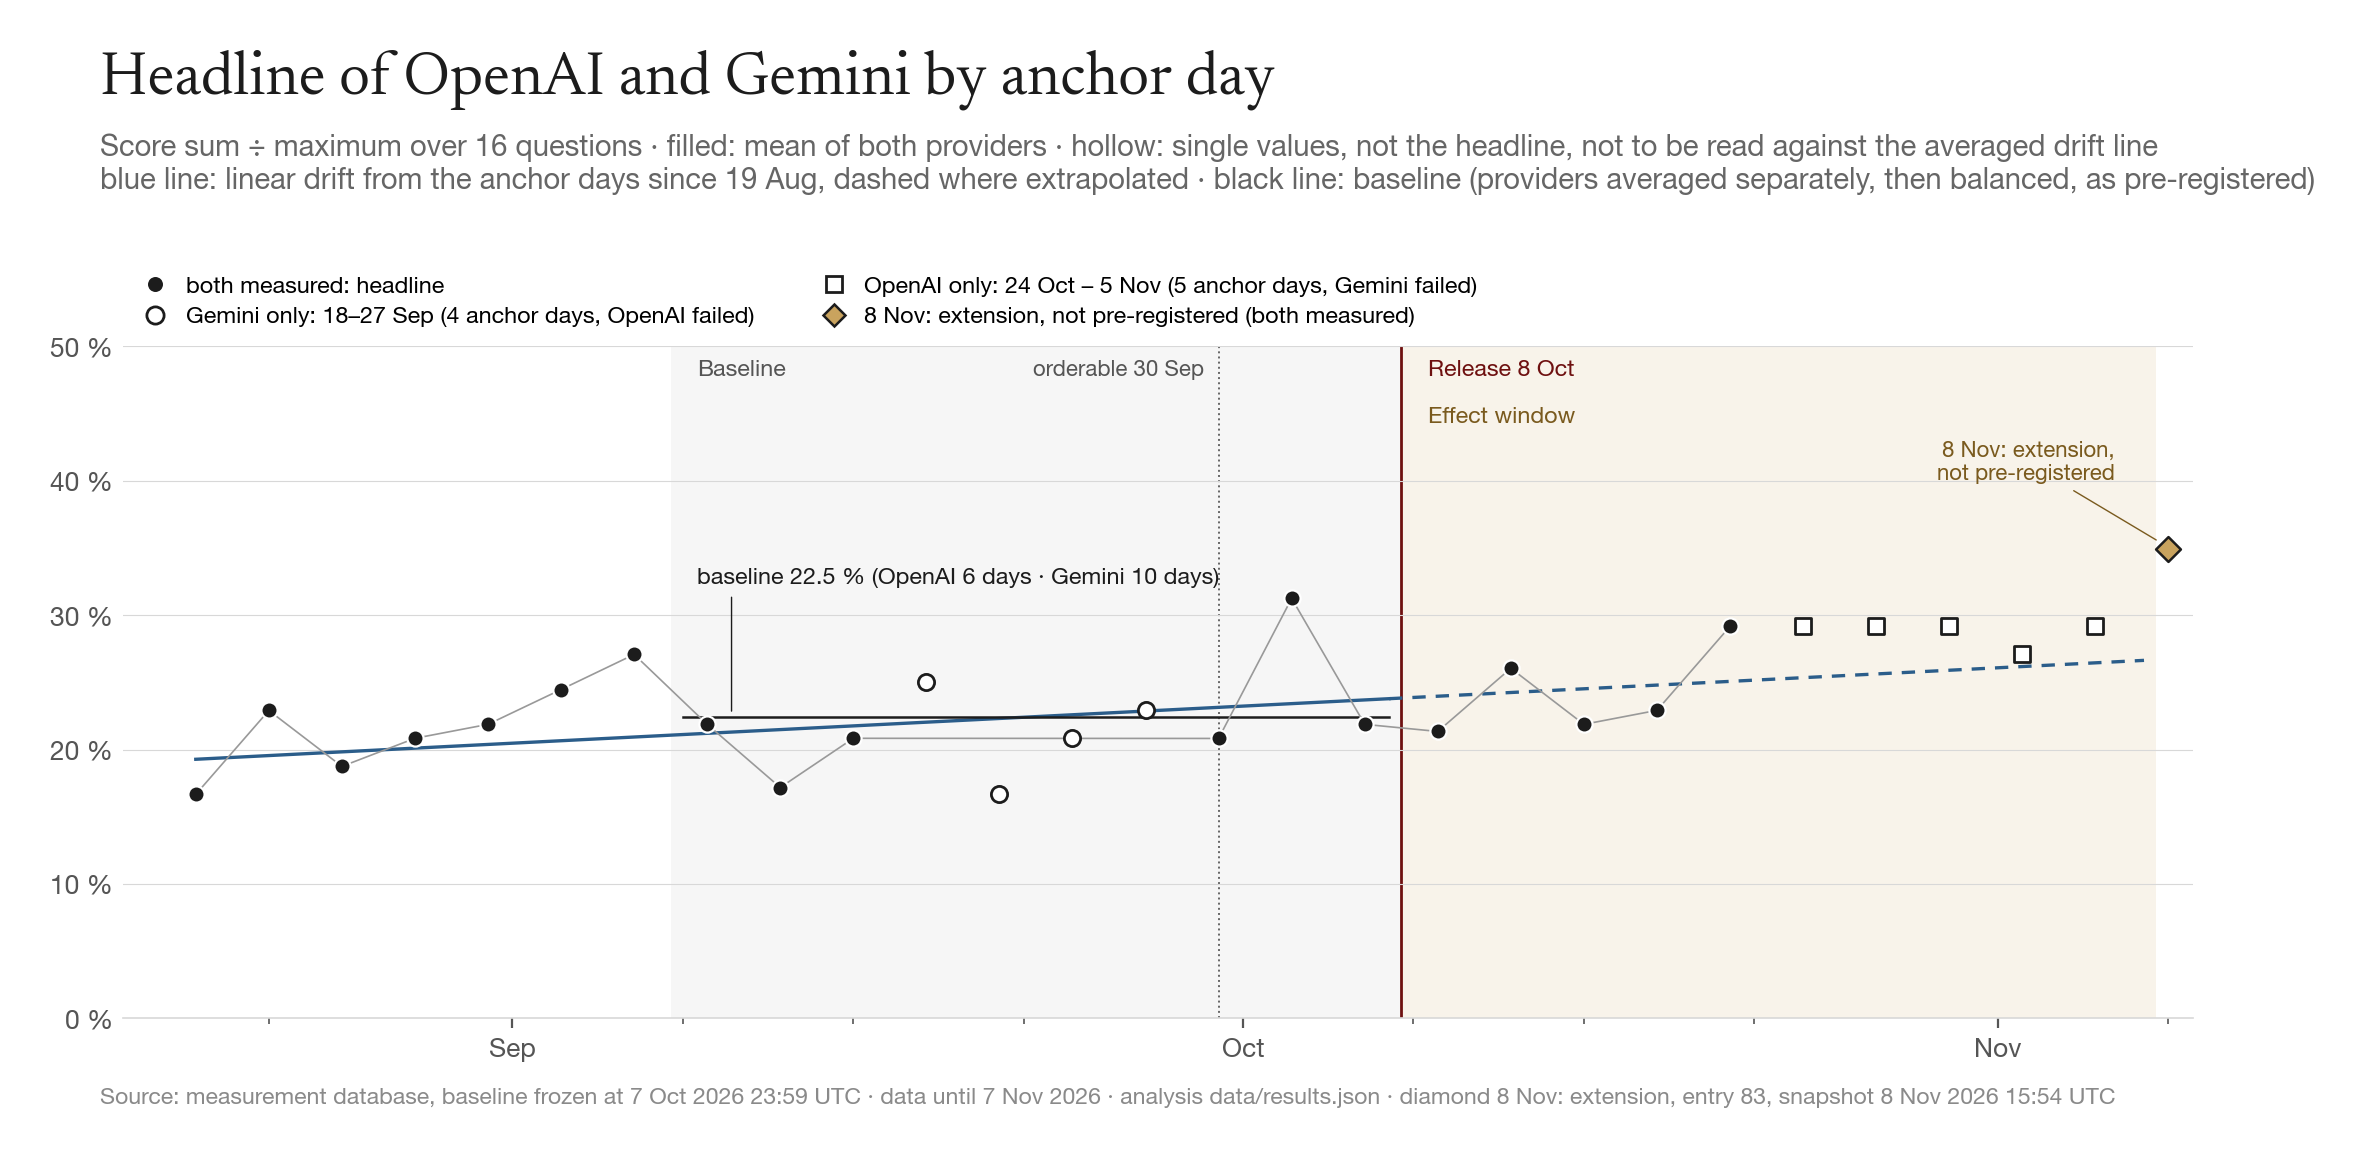
\includegraphics[width=\linewidth]{../figures/fig1_headline_en.png}
\caption*{\textbf{Figure~1:} Headline of OpenAI and Gemini by anchor day with baseline mean, linear drift (dashed where extrapolated) and the marks 30~September (orderable) and 8~October (release). Filled dots are the mean of both providers. Hollow circles mark days on which only Gemini was measured, hollow squares days on which only OpenAI was measured; they are single values, not the headline, and are not to be read against the averaged drift line. The diamond on 8~November is the anchor day from the extension that was not pre-registered (entry~83); baseline and drift of the main analysis are unaffected by it.}\end{figure}

On the 5~anchor days with both providers the headline was 21.35 (9~October), 26.05 (12~October), 21.88 (15~October), 22.92 (18~October), 29.17 (21~October), 24.27~percent on average. On the 5 following anchor days only OpenAI measures (29.17, 29.17, 29.17, 27.08, 29.17); no headline is defined for these days. In the effect window OpenAI averaged 25.62~percent (10~days), Gemini 26.04 (5~days). Drift-adjusted, the difference is +2.22~percentage~points for OpenAI (−4.82~to 8.78), +0.53 for Gemini (−6.33~to 8.84) and +1.38 on average (−3.59~to 6.68). Unadjusted it is +1.67, +5.10 and +3.38 on average (0.05~to 6.93). The interval of the adjusted difference includes zero; the null hypothesis is not rejected. The interval of the unadjusted difference lies just above zero; without amendment~4 it includes zero (section~7). An additional check, not pre-registered, with 200 further seeds of the random number generator shows how narrow this is: the lower bound of the unadjusted interval ranges from −0.07~to 0.17 (0.05 on average) and lies above zero for 157 of the 200~seeds. With 10,000~draws, whether the unadjusted interval excludes zero therefore depends on the seed. The adjusted interval includes zero for every seed (lower bound −3.63~to −3.31, upper bound 6.44~to 6.88). The gap between the unadjusted and the adjusted difference (2.00~percentage~points) is, up to rounding, the drift extended over the effect days actually measured (2.01); under the pre-registration the adjusted difference is the one that counts. The one-sided CUSUM of the headline raises an upward alarm on 5~November. Residuals range from −2.65~to 4.09 on the days with both providers and from 3.88~to 6.02~percentage~points on the days with OpenAI alone; the alarm thus coincides with the basis change (assessment in section~7). No day exceeds the 95~percent prediction~\mbox{limit.}

\Needspace{6\baselineskip}\section{Channels and the hypothesis Direct before Recommendation}

\begin{figure}[htbp]\centering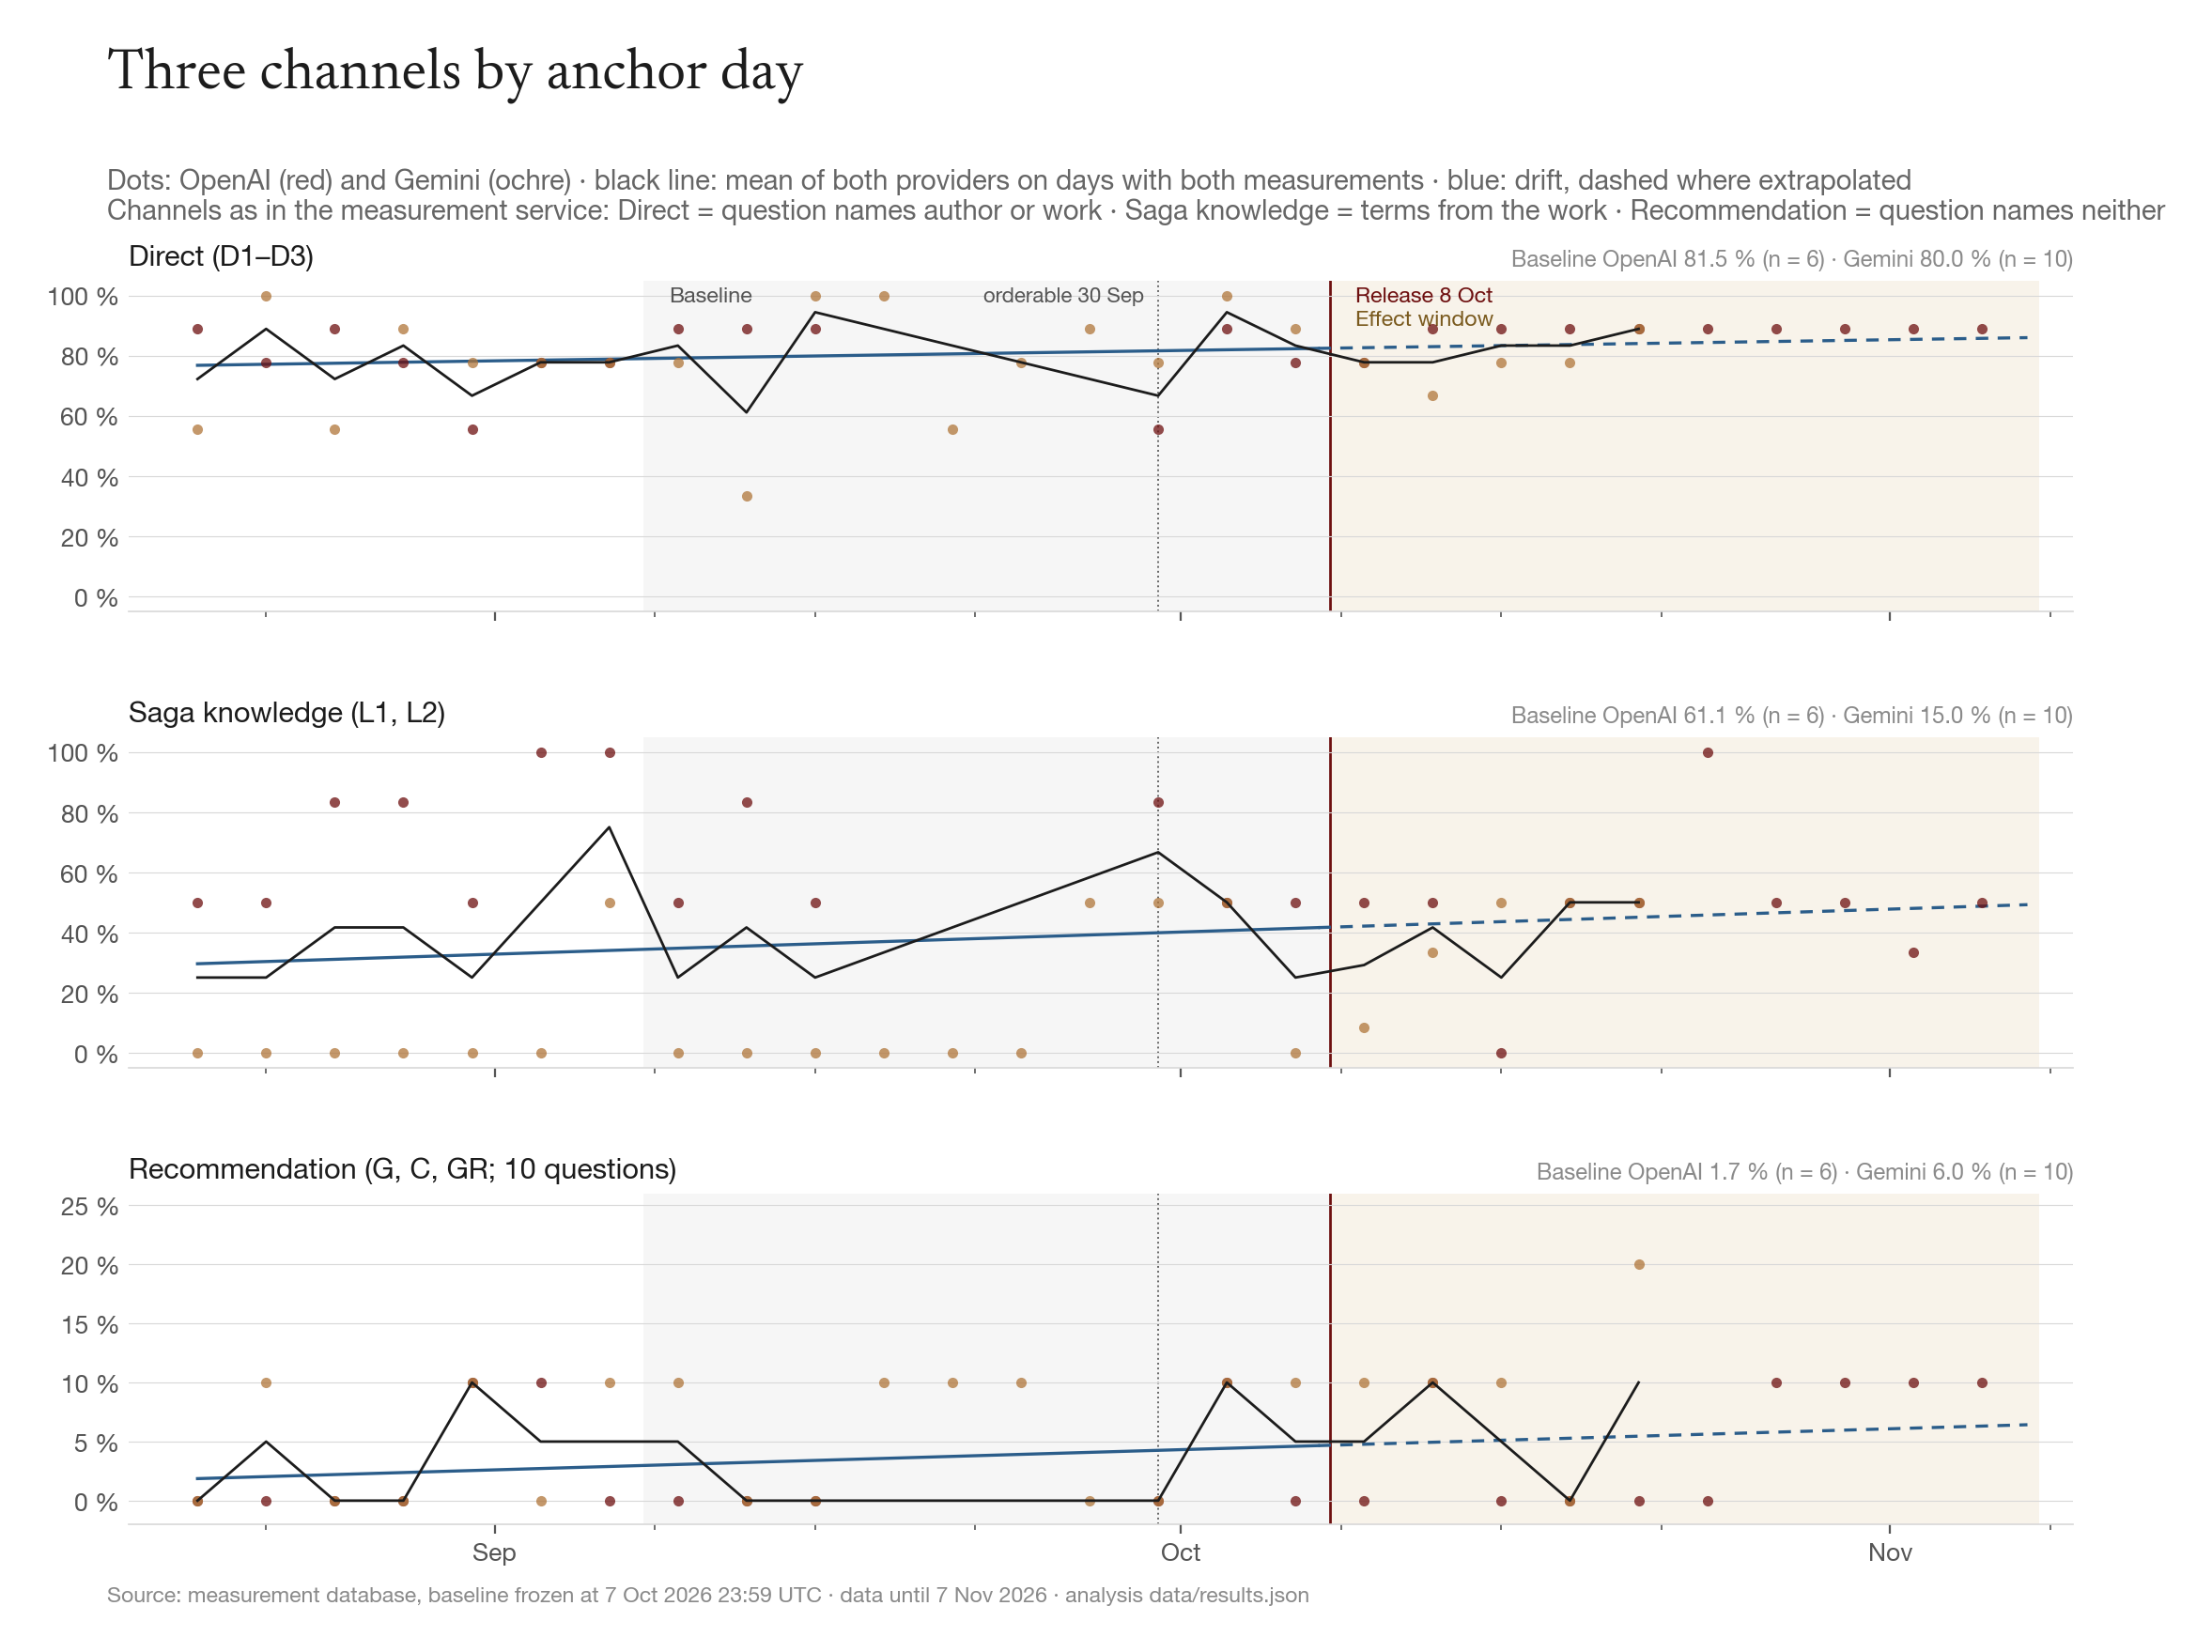
\includegraphics[width=\linewidth]{../figures/fig2_channels_en.png}
\caption*{\textbf{Figure~2:} The three channels Direct, Saga knowledge and Recommendation by anchor day, OpenAI and Gemini separately and averaged.}\end{figure}

Range of the channels on the anchor days of the effect window, percent of the maximum score: OpenAI (10~days): Direct 77.78~to 88.89 (mean 87.78), Saga knowledge 0.00~to 100.00 (mean 48.33), Recommendation 0.00~to 10.00 (mean 5.00); Gemini (5~days): Direct 66.67~to 88.89 (mean 77.78), Saga knowledge 8.33~to 50.00 (mean 38.33), Recommendation 0.00~to 20.00 (mean 10.00). The Saga knowledge channel has only two questions and therefore moves in steps of up to 50~percentage~points. In the Recommendation channel every answer above zero has full points, so 10~percent equals one of the ten answers. OpenAI reaches at most 10~percent there, Gemini at most~\mbox{20.}

\begin{figure}[htbp]\centering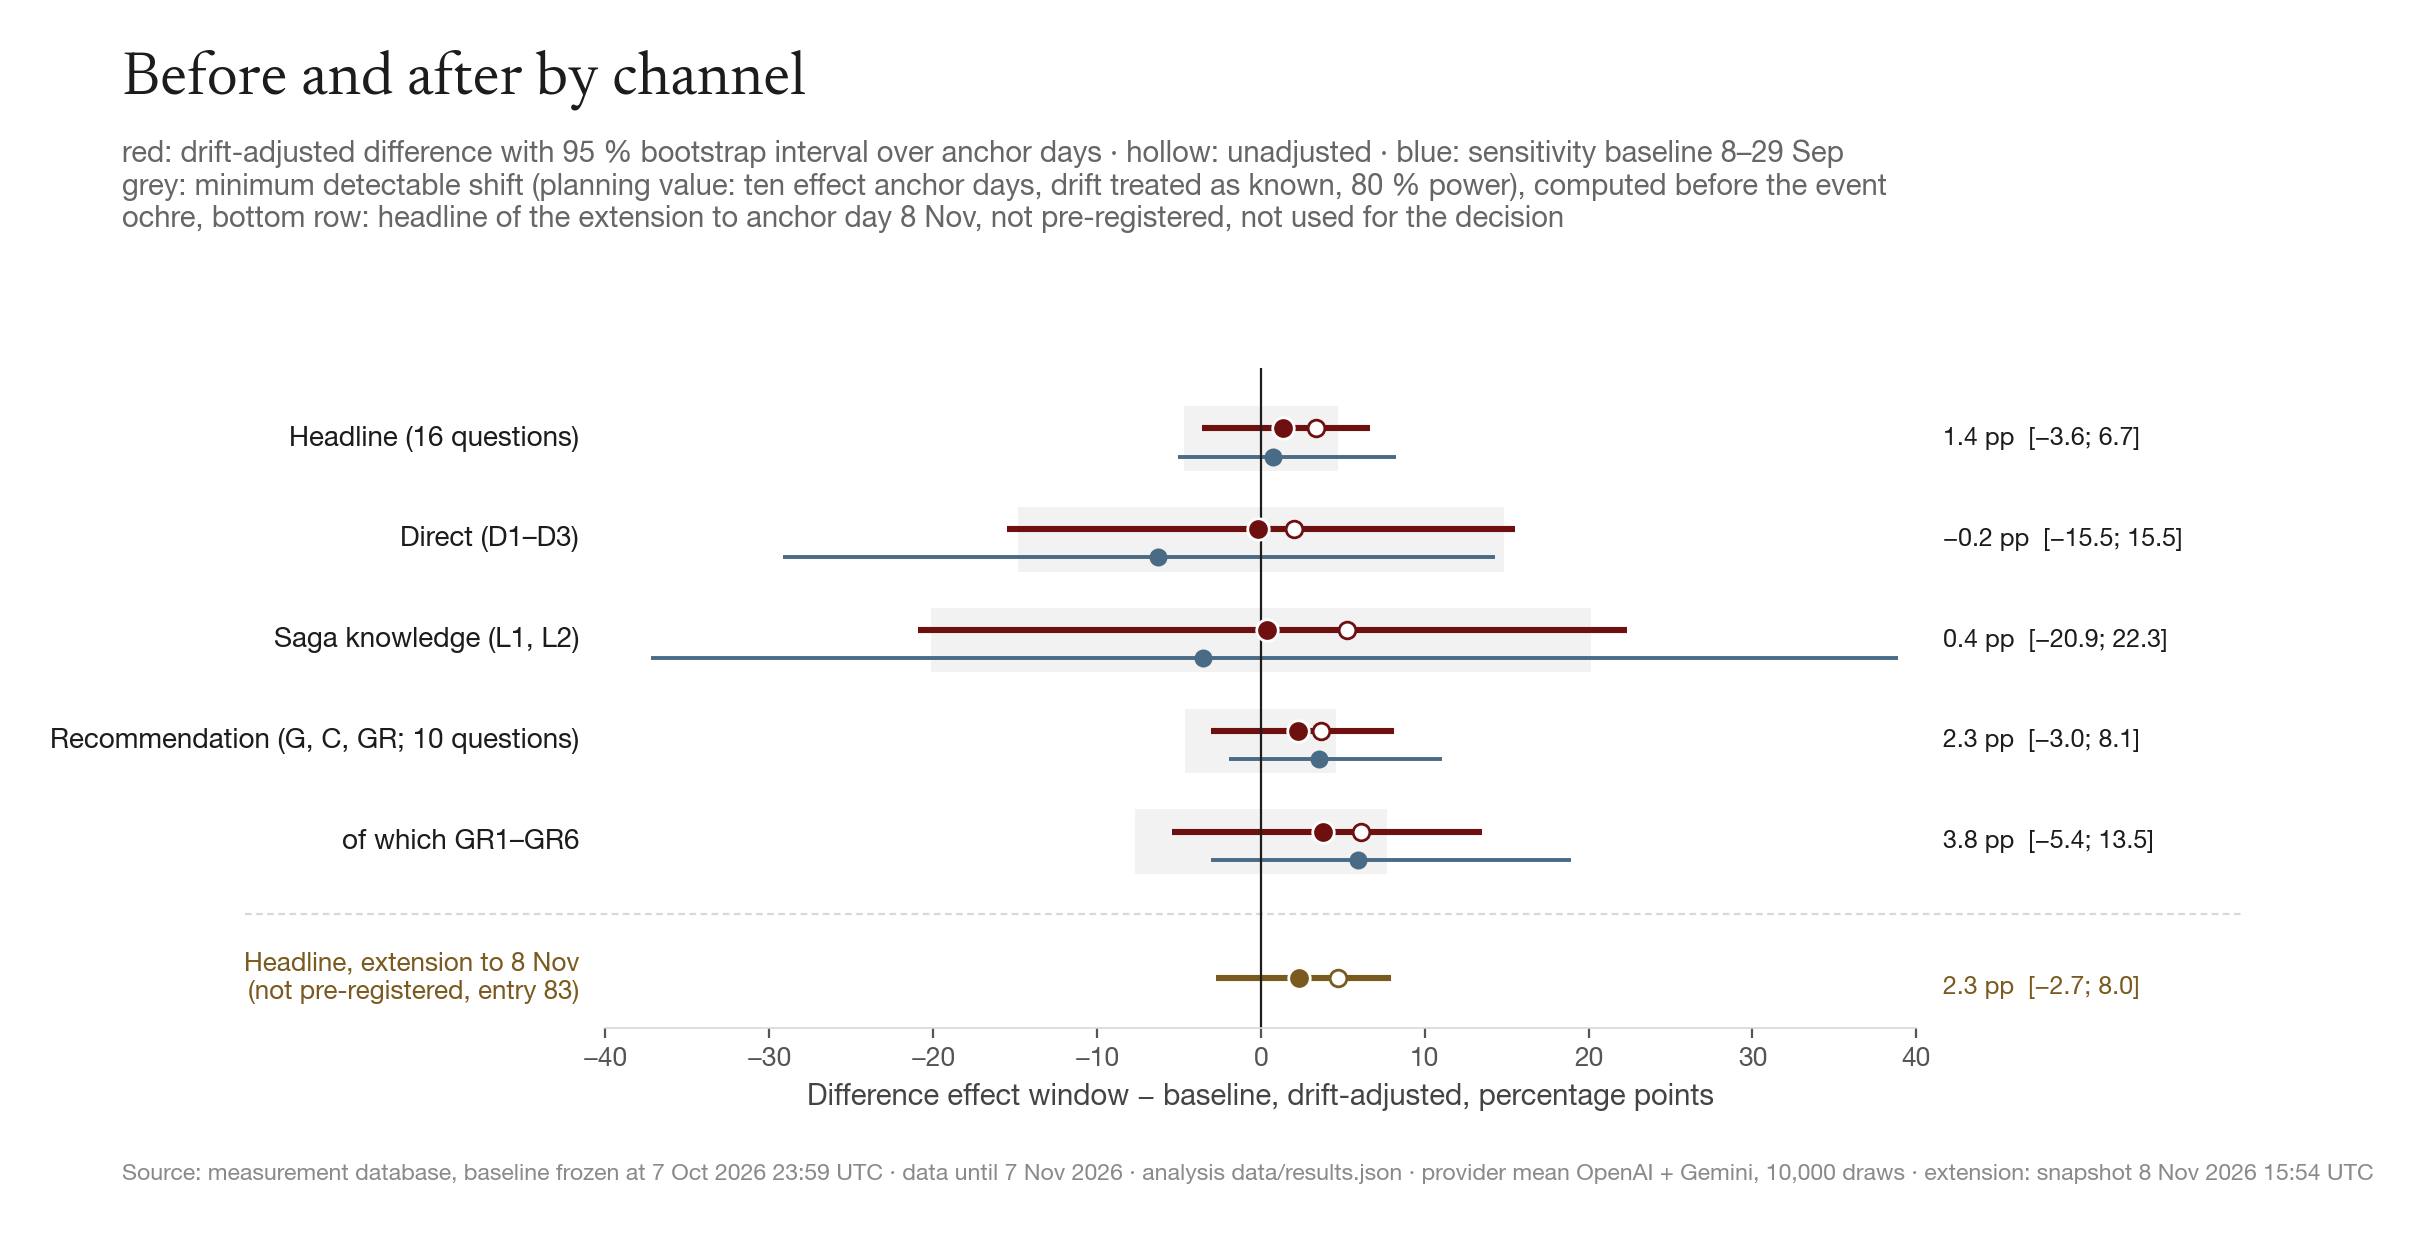
\includegraphics[width=\linewidth]{../figures/fig3_effects_en.png}
\caption*{\textbf{Figure~3:} Before-after differences by channel, drift-adjusted with 95 \% bootstrap interval, unadjusted and against the sensitivity baseline; grey: minimum detectable shift computed before the event (planning value, drift treated as known). The separate bottom row shows the headline of the extension to anchor day 8~November, which was not pre-registered (entry~83); it is not used for the decision.}\end{figure}

\begin{table}[htbp]\centering\footnotesize\setlength{\tabcolsep}{4pt}
\caption*{\normalsize\textbf{Table~4:} Drift-adjusted difference effect window minus baseline by channel, mean of OpenAI and Gemini, percentage~points, with 95 \% bootstrap interval; first deviation by CUSUM and by prediction~\mbox{bound.}}
\begin{tabular}{llllll}\toprule
\makecell[lb]{Channel} & \makecell[lb]{Difference} & \makecell[lb]{95 \% interval} & \makecell[lb]{unadjusted} & \makecell[lb]{first alarm} & \makecell[lb]{first\\exceedance} \\\midrule
\mbox{Headline} & \mbox{+1.38} & \mbox{[−3.59, 6.68]} & \mbox{+3.38} & \mbox{2026-11-05} & \mbox{none} \\
\mbox{Direct} & \mbox{−0.19} & \mbox{[−15.51, 15.53]} & \mbox{+2.04} & \mbox{none} & \mbox{none} \\
\mbox{Saga knowledge} & \mbox{+0.37} & \mbox{[−20.94, 22.34]} & \mbox{+5.27} & \mbox{none} & \mbox{none} \\
\mbox{Recommendation} & \mbox{+2.27} & \mbox{[−3.02, 8.11]} & \mbox{+3.67} & \mbox{none} & \mbox{none} \\
\mbox{of which GR1–GR6} & \mbox{+3.79} & \mbox{[−5.42, 13.48]} & \mbox{+6.12} & \mbox{none} & \mbox{none} \\
\bottomrule\end{tabular}\end{table}

Neither of the two channels that decide the order hypothesis raises an alarm in the effect window, by CUSUM or by the prediction limit; the hypothesis that the Direct channel responds before the Recommendation channel therefore receives no support. The verdict is the same with the pre-registered Recommendation channel GR1~to~GR6. All estimates lie below the planning values of the minimum detectable shift of their channel (headline 4.68, Direct 14.84, Saga knowledge 20.12, Recommendation 4.61, GR1~to~GR6 7.68) and below the values that include the drift uncertainty (section~3); the largest absolute value is 3.79~percentage~points. The design cannot distinguish an effect of this size from zero. The OpenAI and Gemini differences have opposite signs in the Direct channel (OpenAI +9.20, Gemini −9.58) and in the Saga knowledge channel (OpenAI −7.90, Gemini~\mbox{+8.63).}

\Needspace{6\baselineskip}\section{Claude, descriptive}

\begin{figure}[htbp]\centering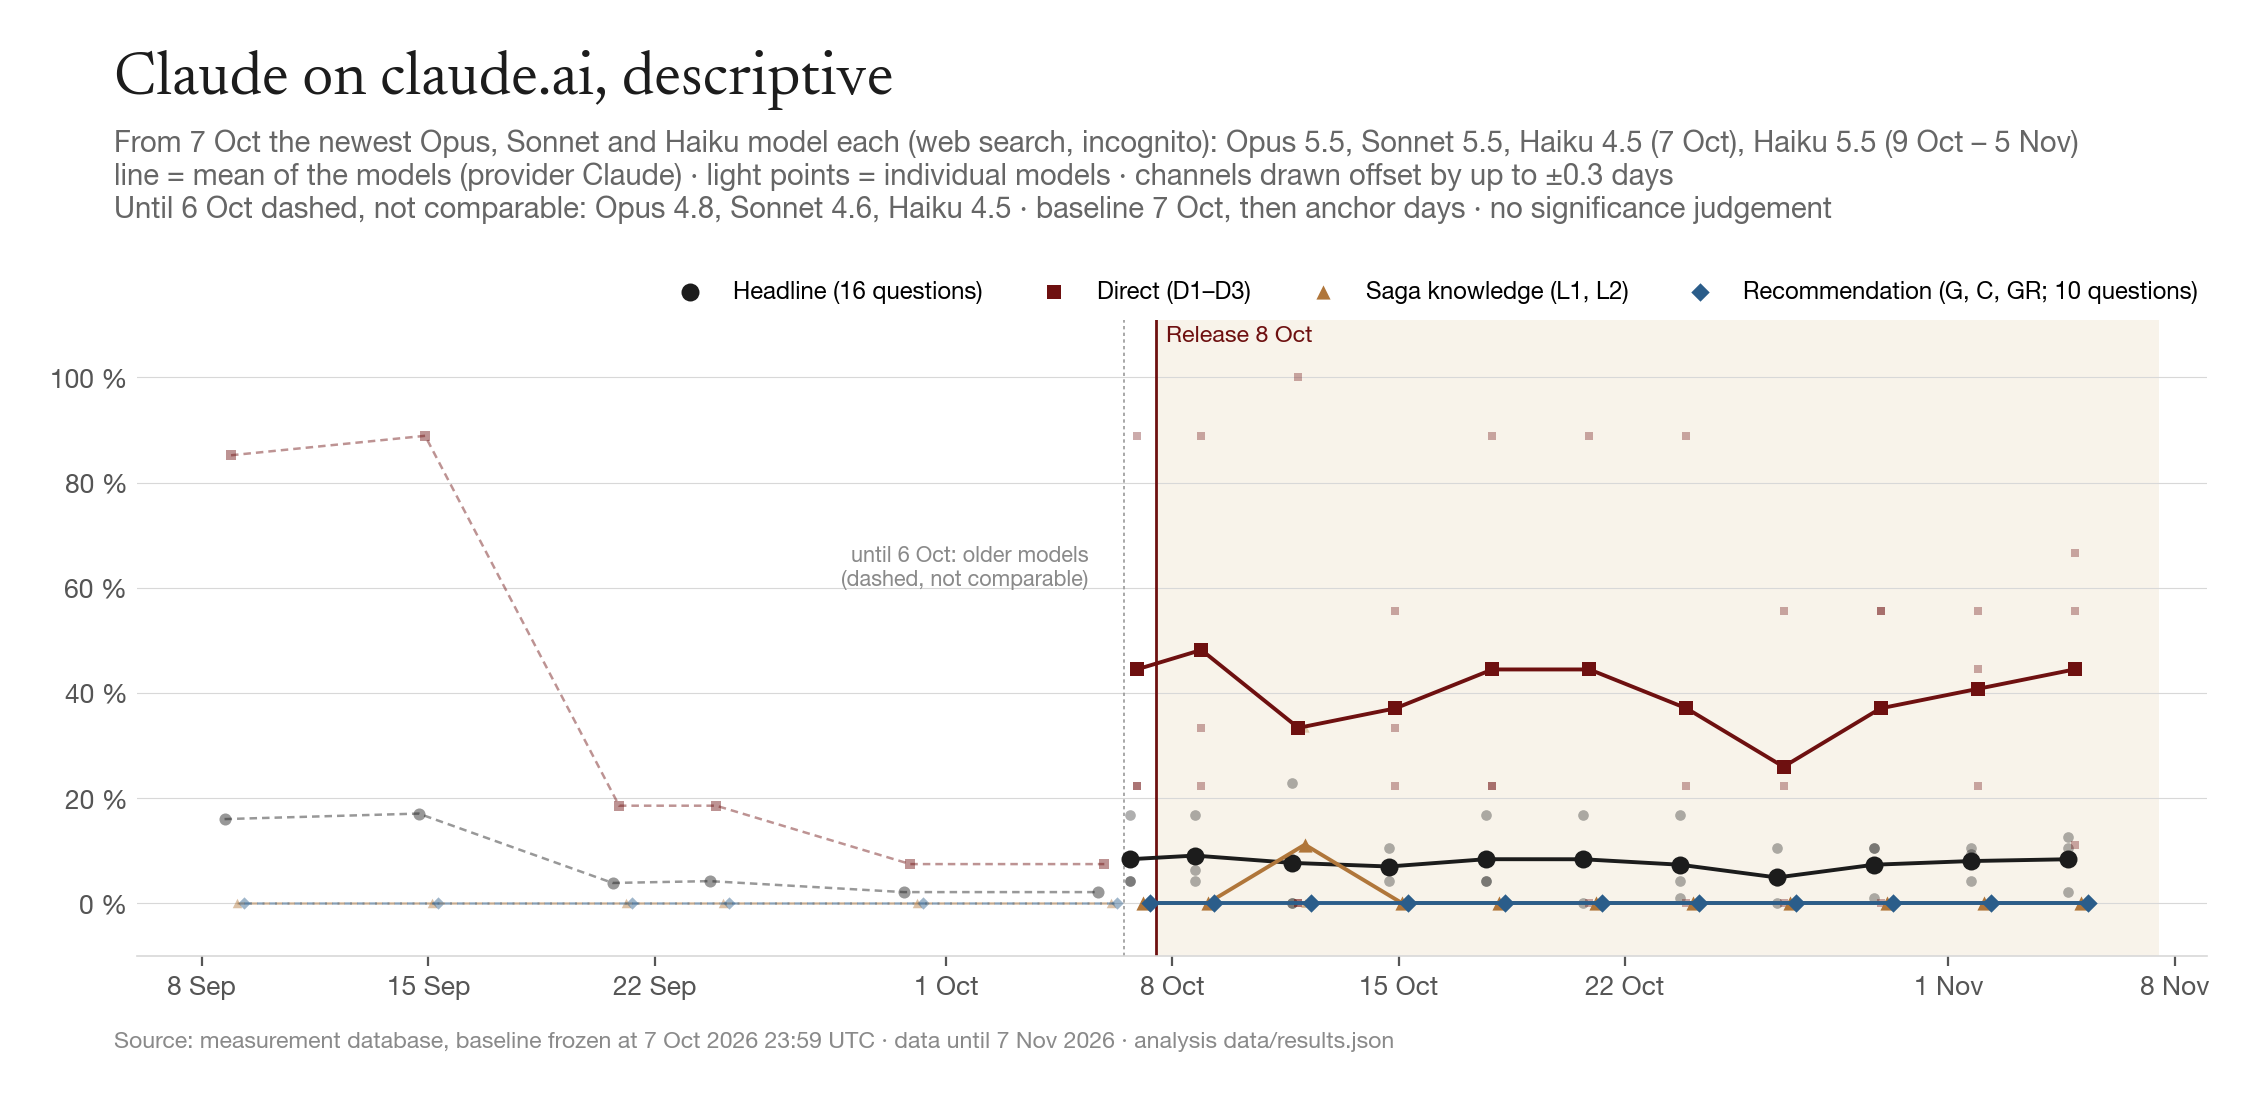
\includegraphics[width=\linewidth]{../figures/fig4_claude_en.png}
\caption*{\textbf{Figure~4:} Claude on claude.ai, descriptive: the newest Opus, Sonnet and Haiku model each in an incognito chat with web search (entry~41). The line is the mean of the three models, the light points are the individual models. Dashed is the older, non-comparable series until 6~October. Baseline measurement on 7~October, anchor days from 9~October; the channels are drawn offset by up to 0.3~days.}\end{figure}

Each family was measured with its newest model: \mbox{claude-haiku-4-5-20251001}, \mbox{claude-opus-5-5}, \mbox{claude-sonnet-5-5} in the baseline measurement on 7~October, \mbox{claude-haiku-5-5}, \mbox{claude-opus-5-5}, \mbox{claude-sonnet-5-5} from 9~October. For Haiku the model therefore changed between baseline and first anchor day (entries~45~and 49); Opus and Sonnet stayed the same. Each day has 48 of 48~answers with values; the register lists no Claude outage in the effect~\mbox{window.}

\begin{table}[htbp]\centering\footnotesize\setlength{\tabcolsep}{4pt}
\caption*{\normalsize\textbf{Table~5:} Claude on claude.ai per measurement day: mean of the three models per channel and daily value per model, percent of the maximum~\mbox{score.}}
\begin{tabularx}{\linewidth}{>{\raggedright\arraybackslash}Xlllllll}\toprule
Day & \makecell[lb]{Claude\\headline} & \makecell[lb]{Direct} & \makecell[lb]{Saga\\knowledge} & \makecell[lb]{Recommendation} & \makecell[lb]{Opus} & \makecell[lb]{Sonnet} & \makecell[lb]{Haiku} \\\midrule
2026-10-07 \mbox{(baseline)} & \mbox{8.34} & \mbox{44.44} & \mbox{0.00} & \mbox{0.00} & \mbox{16.67} & \mbox{4.17} & \mbox{4.17} \\
2026-10-09 & \mbox{9.03} & \mbox{48.15} & \mbox{0.00} & \mbox{0.00} & \mbox{16.67} & \mbox{4.17} & \mbox{6.25} \\
2026-10-12 & \mbox{7.64} & \mbox{33.33} & \mbox{11.11} & \mbox{0.00} & \mbox{22.92} & \mbox{0.00} & \mbox{0.00} \\
2026-10-15 & \mbox{6.95} & \mbox{37.04} & \mbox{0.00} & \mbox{0.00} & \mbox{10.42} & \mbox{4.17} & \mbox{6.25} \\
2026-10-18 & \mbox{8.34} & \mbox{44.44} & \mbox{0.00} & \mbox{0.00} & \mbox{16.67} & \mbox{4.17} & \mbox{4.17} \\
2026-10-21 & \mbox{8.33} & \mbox{44.44} & \mbox{0.00} & \mbox{0.00} & \mbox{16.67} & \mbox{8.33} & \mbox{0.00} \\
2026-10-24 & \mbox{7.29} & \mbox{37.04} & \mbox{0.00} & \mbox{0.00} & \mbox{16.67} & \mbox{4.17} & \mbox{1.04} \\
2026-10-27 & \mbox{4.86} & \mbox{25.93} & \mbox{0.00} & \mbox{0.00} & \mbox{10.42} & \mbox{4.17} & \mbox{0.00} \\
2026-10-30 & \mbox{7.29} & \mbox{37.04} & \mbox{0.00} & \mbox{0.00} & \mbox{10.42} & \mbox{10.42} & \mbox{1.04} \\
2026-11-02 & \mbox{7.99} & \mbox{40.74} & \mbox{0.00} & \mbox{0.00} & \mbox{10.42} & \mbox{4.17} & \mbox{9.38} \\
2026-11-05 & \mbox{8.33} & \mbox{44.45} & \mbox{0.00} & \mbox{0.00} & \mbox{12.50} & \mbox{10.42} & \mbox{2.08} \\
\bottomrule\end{tabularx}\end{table}

In the baseline measurement the daily value was 8.34~percent (Opus 16.67, Sonnet 4.17, Haiku 4.17). On the anchor days it ranged from 4.86~to 9.03, the Direct channel from 25.93~to 48.15. Saga knowledge was above zero only on 12~October (11.11), Recommendation on no day. On the last anchor day, 5~November, the difference to the baseline measurement is −0.01~percentage~points on average (Direct +0.01); per model Opus −4.17, Sonnet +6.25, Haiku −2.09. The Claude values, too, follow the scorer in its pre-registered version throughout; on 5~November the Sonnet answer to question D1 therefore counts with zero points after re-scoring on the full text. It describes the author correctly and distinguishes him from Pauline Kael at the end; the same holds for the answers of Opus and Sonnet on 30~October and 2~November (section~1). Under the wording of entry~43 each of these answers would score one point. The daily value as the mean of the three models, in percent, would then be 8.68 instead of 7.29 on 30~October, 9.38 instead of 7.99 on 2~November and 9.03 instead of 8.33 on 5~November; Sonnet would be at 12.50 instead of 10.42~percent on 5~November. There is no significance statement for Claude. Claude's daily values are below those of OpenAI and Gemini on every~\mbox{day.}

\Needspace{6\baselineskip}\section{Robustness and sensitivity}

\begin{figure}[htbp]\centering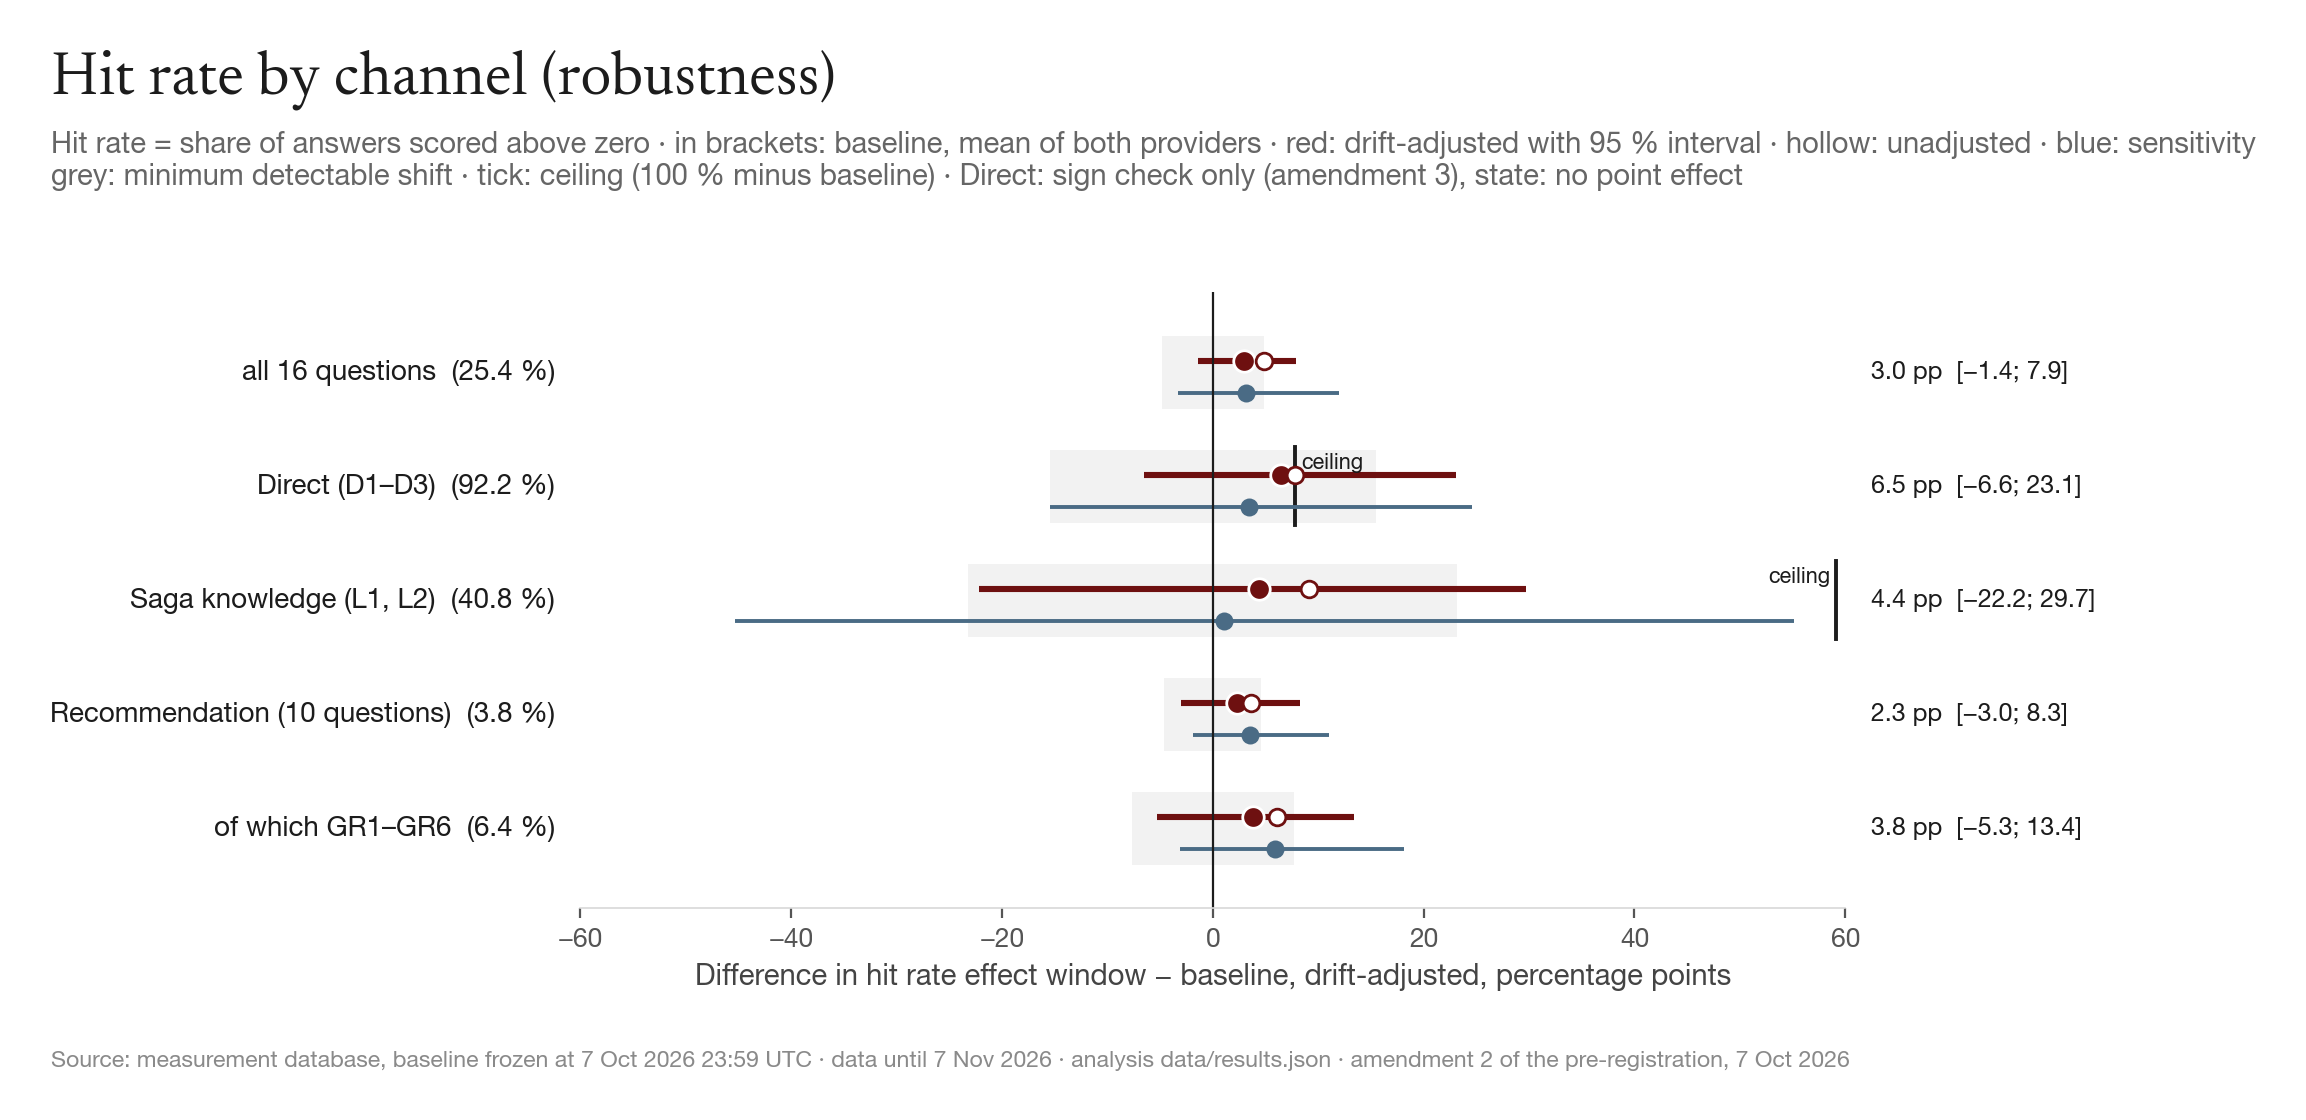
\includegraphics[width=\linewidth]{../figures/fig5_hitrate_en.png}
\caption*{\textbf{Figure~5:} Hit rate (share of answers scored above zero) by channel: baseline, drift-adjusted difference with 95 \% bootstrap interval, sensitivity baseline, minimum detectable shift and ceiling at 100~percent; in the Direct channel the hit rate serves as a sign check only (amendment~3).}\end{figure}

Hit rate, drift-adjusted difference effect window minus baseline, mean of both providers (percentage~points, 95 \% interval): all questions +2.95 (−1.40~to 7.85), Direct +6.45 (−6.55~to 23.09), Saga knowledge +4.42 (−22.16~to 29.72), Recommendation +2.27 (−2.97~to 8.29), GR1~to~GR6 +3.79 (−5.26~to 13.42). All intervals include zero. Like the headline, the CUSUM of the hit rate across all questions raises an upward alarm on 5~November, a day with OpenAI alone; the channels raise none, their highest CUSUM sum lies between 0.70~and 3.68 at the threshold 5. Under the interval rule no channel shows a robust effect, because the intervals of the point differences already include zero. In the Direct channel there is no point effect to check under amendment~3; the hit-rate estimate (+6.45) is therefore not read as~\mbox{confirmation.}

Against the sensitivity baseline of 8 to 29~September (OpenAI 3, Gemini 7~anchor days) the drift-adjusted differences are: headline +0.74 (−5.08~to 8.22), Direct −6.27 (−29.18~to 14.27), Saga knowledge −3.54 (−37.24~to 38.88), Recommendation +3.55 (−1.96~to 11.06), GR1~to~GR6 +5.92 (−3.06~to 18.90). Here too no interval of the two-provider mean excludes zero. For single providers only these drift-adjusted intervals exclude zero, all against the sensitivity baseline: OpenAI, Recommendation in points +5.00 (0.86~to 15.36); OpenAI, GR1~to~GR6 in points +8.33 (1.52~to 27.02); Gemini, hit rate all questions +7.36 (0.89~to 16.80); Gemini, hit rate Saga knowledge +30.99 (0.98~to 55.49); OpenAI, hit rate Recommendation +5.00 (0.81~to 15.91); OpenAI, hit rate GR1~to~GR6 +8.33 (1.50~to 25.94). The pre-registered decision rests on the mean of both providers. Without drift removal, the intervals for headline +3.38 (0.05~to 6.93) and hit rate all questions +4.89 (2.08~to 7.71) exclude zero in the main analysis, and those for headline +4.23 (0.97~to 7.77), Recommendation +4.64 (0.93~to 8.36), GR1~to~GR6 +7.73 (1.67~to 13.93), hit rate all questions +6.05 (3.05~to 8.93), hit rate Recommendation +4.64 (1.00~to 8.36) and hit rate GR1~to~GR6 +7.73 (1.55~to 13.93) against the sensitivity baseline; for the headline of the main analysis this depends on the seed (section~4). Under the pre-registration the drift-adjusted difference is the one that counts; drift adjustment reduces each of these values. With the scoring rules of 2~November applied to baseline and effect window (entry~71) the results are headline +2.77 (−2.37~to 8.28), Direct +4.22 (−10.31~to 19.31) and Saga knowledge +4.75 (−18.83~to 27.93); the headline baseline is then 21.59 instead of 22.45~percent. In drift base and baseline the new rules were applied to the stored 500-character excerpt only. This changes 41 stored answers: 18 from OpenAI and Gemini, 22 from the earlier Claude series and one from the Claude baseline measurement of 7~October. Of these, 9 enter the OpenAI and Gemini metrics because they lie on anchor days (Gemini 8, OpenAI 1); the other 9 lie on intermediate days, which are not analysed (section~2). Before 15~September the then valid release date of 22~September still counts. Under these rules the CUSUM of the headline raises an alarm as early as 30~October. The decision is unchanged. Comparing the baseline holdings with the pull of 8~November finds no missing, changed or new rows (section~2).

Empty answers. Before 1~November they enter as answers without a finding, with zero points (entry~66). On the anchor days these are 19~answers, all from Gemini: 7 in the drift base, 7 in the baseline and 5 in the effect window; OpenAI gave no empty answer on anchor days. Treated as gaps, the question is missing on that day and the daily value is formed from the remaining questions. The headline difference is then +1.70 (−3.27~to 6.96), unadjusted +3.77 (0.51~to 7.13); Direct −0.19 (−15.51~to 15.53), Saga knowledge +0.37 (−20.94~to 22.34), Recommendation +2.42 (−3.01~to 8.38), GR1~to~GR6 +4.62 (−4.74~to 14.43). Neither the headline nor any channel or hit rate raises an alarm, so the alarm of the main analysis on 5~November disappears, and the decision is unchanged. Treated as failed measurements, the provider-day is incomplete and drops out. Gemini then keeps 2~anchor days in the drift base, 5 in the baseline and one in the effect window (21~October); no interval can be computed for Gemini, and the headline estimate as the mean of both providers (+11.23) cannot be interpreted. In this variant the CUSUM of the headline and of the hit rate across all questions raises an alarm on 30~October, those of the Recommendation channel and of questions GR1~to~GR6 on 5~November; the Direct channel raises none. The Recommendation channel thus responds before the Direct channel, and the order hypothesis receives no support here either. This variant is not informative because so few Gemini days~\mbox{remain.}

Without amendment~4. If the two answers of 12~October that were changed retroactively on 15~October count with zero points again, the headline difference is +0.96 (−4.15~to 6.36), unadjusted +2.97 (−0.62~to 6.72), and −2.97 (−25.11~to 19.75) in the Saga knowledge channel; Direct, Recommendation and GR1~to~GR6 are unchanged. In the main analysis the unadjusted headline interval therefore excludes zero only because of this one Gemini answer, and even then not for every seed (section~4). The CUSUM alarm of the headline on 5~November remains, and the decision does not change. The full texts of all 57 OpenAI and Gemini answers that score above zero under the pre-registered rules on the anchor days from 18~October to 8~November were reviewed. 54 name the author, 2 Direct answers to question D3 identify him through the domain, and one OpenAI answer to question R1 of 8~November receives half a point because it repeats the word Marin from the question; under the values in the measurement database it scores zero, and there are 56~answers. No further answer therefore depends on the title as anchor alone; for D2 and D3 the title anchor does not apply anyway. This was not checked for~\mbox{Claude.}

Additional figures, not pre-registered. Restricted to the 5~anchor days with both providers (9~October to 21~October) the headline is −0.26 (−4.96~to 4.82) drift-adjusted and +1.82 (−1.68~to 5.52) unadjusted; the positive estimate of the main analysis thus comes from the later days on which OpenAI measures alone. Against its own drift line OpenAI averages −1.04~percentage~points in the first half of the effect window (9~October to 21~October) and +5.49 in the second (24~October to 5~November). The CUSUM alarm of the headline on 5~November is narrow: the highest sum is 5.25 at the threshold 5. It occurs only while the standard deviation used for standardisation is below 3.941; the value used, computed from the baseline by the procedure fixed in advance, is 3.821. Under the scoring rules of 2~November the headline raises an alarm as early as 30~October. The decision on the null hypothesis does not depend on this~\mbox{alarm.}

The delayed-effect observation covers 20~anchor days from 8~November to 4~January~2027. None of them is analysed in the main analysis; only the extension in the following subsection, which is not pre-registered, counts the first of them, 8~November, as part of the effect window. The observation will be frozen after 6~January~2027 and reported descriptively as an addendum; it does not lead to a new significance~\mbox{statement.}

\Needspace{6\baselineskip}\subsection{Extension to anchor day 8~November (not pre-registered)}

After the effect window had closed I decided to report, in addition to the pre-registered main analysis, an extension of the effect window up to and including anchor day 8~November (entry~83). The reason is the Gemini measurement of that day: Gemini was missing on the last five anchor days of the effect window and is measured again on 8~November. The extension is not pre-registered. Hypothesis, null hypothesis, metrics, drift removal, scoring rules and decision rule are unchanged, and the hypotheses are decided by the main analysis alone, with the effect window ending on 7~November. Under the pre-registration, 8~November belongs to the delayed-effect observation. On the morning of 8~November both interfaces refused every question (entries~80~and 81). OpenAI was re-measured at 14:24~UTC under the catch-up rule of entry~44, and Gemini at 15:48~UTC under the catch-up rule of entry~82, which was recorded on the same day at 14:30~UTC before its first use. The extension itself was recorded in the register at 15:52~UTC, after both re-measurements; it should therefore be read as a post-hoc analysis. The Gemini gaps from 24~October to 5~November are not re-measured. The basis is the third pull of 8~November (section~2). The 80~answers of 8~November are scored on the full text under the pre-registered rules; three of them differ from the value in the measurement database, none from Gemini, and together with the eleven of the main analysis the extension resets 14~answers. The procedure and the seed are the same as in the main~\mbox{analysis.}

\begin{table}[htbp]\centering\footnotesize\setlength{\tabcolsep}{4pt}
\caption*{\normalsize\textbf{Table~6:} Extension of the effect window to anchor day 8~November, not pre-registered: drift-adjusted difference to the baseline, mean of OpenAI and Gemini, percentage~points, compared with the main analysis; 95 \% bootstrap interval, unadjusted difference and first CUSUM alarm in the~\mbox{extension.}}
\begin{tabularx}{\linewidth}{>{\raggedright\arraybackslash}Xllllll}\toprule
Channel & \makecell[lb]{Main analysis} & \makecell[lb]{Extension} & \makecell[lb]{95 \% interval} & \makecell[lb]{unadjusted} & \makecell[lb]{95 \% interval\\unadjusted} & \makecell[lb]{first alarm} \\\midrule
Headline & \mbox{+1.38} & \mbox{+2.32} & \mbox{[−2.74, 7.95]} & \mbox{+4.72} & \mbox{[1.03, 8.60]} & \mbox{2026-11-05} \\
Direct & \mbox{−0.19} & \mbox{+1.13} & \mbox{[−14.70, 17.46]} & \mbox{+3.94} & \mbox{[−4.63, 13.52]} & \mbox{none} \\
Saga knowledge & \mbox{+0.37} & \mbox{+4.39} & \mbox{[−18.50, 29.14]} & \mbox{+10.49} & \mbox{[−5.20, 26.72]} & \mbox{none} \\
Recommendation & \mbox{+2.27} & \mbox{+2.31} & \mbox{[−3.03, 8.28]} & \mbox{+3.90} & \mbox{[0.44, 7.38]} & \mbox{none} \\
of which GR1–GR6 & \mbox{+3.79} & \mbox{+3.85} & \mbox{[−5.35, 13.64]} & \mbox{+6.49} & \mbox{[0.53, 12.25]} & \mbox{none} \\
Hit rate, all questions & \mbox{+2.95} & \mbox{+3.92} & \mbox{[−0.88, 9.31]} & \mbox{+6.25} & \mbox{[3.01, 9.54]} & \mbox{2026-11-05} \\
\bottomrule\end{tabularx}\end{table}

On 8~November OpenAI stood at 30.21 and Gemini at 39.58~percent, the headline at 34.89~percent. With this day OpenAI contributes 11 and Gemini 6 effect anchor days, and the headline is defined on 6~anchor days. Drift-adjusted, the headline difference is +2.67 (−4.43~to 9.28) for OpenAI, +1.97 (−5.46~to 10.96) for Gemini and +2.32~percentage~points on average (−2.74~to 7.95); unadjusted it is +4.72 (1.03~to 8.60) on average, and the drift extended over the effect days actually measured is 2.40. The interval of the adjusted difference includes zero. In the channels and in the hit rate every drift-adjusted interval of the two-provider mean includes zero (Table~6), also against the sensitivity baseline, where the headline difference is +1.73 (−4.30~to 9.69). For single providers only these drift-adjusted intervals exclude zero, all against the sensitivity baseline: OpenAI, Recommendation in points +5.45 (1.40~to 16.96); OpenAI, GR1~to~GR6 in points +9.09 (2.28~to 27.85); Gemini, hit rate all questions +8.69 (1.64~to 19.78); Gemini, hit rate Saga knowledge +37.56 (4.06~to 75.00); OpenAI, hit rate Recommendation +5.45 (1.42~to 16.08); OpenAI, hit rate GR1~to~GR6 +9.09 (2.24~to 27.95). Without drift removal, the intervals for headline +4.72 (1.03~to 8.60), Recommendation +3.90 (0.44~to 7.38), GR1~to~GR6 +6.49 (0.53~to 12.25), hit rate all questions +6.25 (3.01~to 9.54), hit rate Recommendation +3.90 (0.44~to 7.30) and hit rate GR1~to~GR6 +6.49 (0.66~to 12.17) exclude zero against the baseline, and those for headline +5.57 (1.91~to 9.39), Recommendation +4.87 (1.54~to 8.16), GR1~to~GR6 +8.12 (2.63~to 13.73), hit rate all questions +7.42 (4.19~to 10.89), hit rate Recommendation +4.87 (1.51~to 8.16) and hit rate GR1~to~GR6 +8.12 (2.63~to 13.60) against the sensitivity baseline. As in the main analysis, the drift-adjusted difference of the two-provider mean is the one that counts; drift adjustment reduces each of these values. As in the main analysis, the CUSUM raises an alarm only for the headline and the hit rate across all questions, both on 5~November. Direct and Recommendation raise none, also with GR1~to~GR6, and the order hypothesis receives no support. Under the interval rule no channel shows a robust effect, and in the Direct channel there is no point effect to~\mbox{check.}

Compared with the main analysis the headline estimate rises by 0.94~percentage~points. The interval still includes zero, and the decision on the null hypothesis would be the same. For Gemini a single day is added at the end of the window; the gap from 24~October to 5~November remains, and the Gemini difference still rests on five days in the first half of the window and this one day. Claude stood at 5.90~percent on 8~November as the mean of the three models (Direct 29.63); this value is~\mbox{descriptive.}

\Needspace{6\baselineskip}\section{Deviations from the plan}

Table~7 summarises where this report deviates from the original plan, when the deviation was fixed, where it is recorded in the data-gap register and how it is handled. Amendments 1 to 3 and the rules of 7~October were registered before the event, except for the ten-question Recommendation channel, which was fixed on 7~October before the event in the analysis code only; all later ones are disclosed as such and, where they touch values, accompanied by a sensitivity~\mbox{analysis.}

\begin{table}[htbp]\centering\footnotesize
\caption*{\normalsize\textbf{Table~7:} Deviations from the plan: when fixed, register entry and handling in this~\mbox{report.}}
\begin{tabularx}{\linewidth}{>{\raggedright\arraybackslash\hsize=1.0\hsize}X>{\raggedright\arraybackslash\hsize=0.7\hsize}Xl>{\raggedright\arraybackslash\hsize=1.3\hsize}X}\toprule
Deviation & fixed & \makecell[lb]{Entry} & Handling \\\midrule
Amendments 1 to 3: panel OpenAI and Gemini, Claude descriptive, sensitivity baseline, hit rate, analysis details, Direct rule & 7 Oct, before the event & \mbox{36, 38, 39} & part of the pre-registration \mbox{(sections~1~and 3)} \\
Rules: Claude with three model families, honest non-result & 7 Oct, before the event & \mbox{41, 42} & applied equally to baseline and effect window \mbox{(sections~1~and 2)} \\
Name collision with Pauline Kael; the scorer in its pre-registered version implements the part on genuine statements about the author more narrowly than the wording & 7 Oct, before the event; identified as a fault on 2 Nov & \mbox{43, 71} & before the event one Gemini answer re-scored according to the wording; in the effect window the main analysis follows the scorer: 5 Claude answers \mbox{(6 in the extension)} with zero points, OpenAI and Gemini not affected; Claude values under the wording descriptive \mbox{(sections~1~and 6)} \\
Catch-up rule for OpenAI & 7 Oct, before the event & \mbox{44} & effective only in the effect window (2 Nov; in the extension also 8 Nov), the baseline contains no re-measurement \mbox{(section~2)} \\
Recommendation channel with ten questions instead of GR1~to~GR6 & 7 Oct, in the analysis code, not registered & \mbox{–} & GR1~to~GR6 reported throughout, same verdict \mbox{(sections~2~and 5)} \\
Amendment 4: book or series title as anchor & 15 Oct, during the effect window & \mbox{50} & sensitivity without amendment~4 \mbox{(section~7)} \\
Empty answers as failed measurements, repeat within the same run & 1 Nov and 2 Nov, during the effect window & \mbox{66, 70} & zero points before; sensitivity as gaps and as failed measurements \mbox{(section~7)} \\
Scoring rules of 2~November & 2 Nov, during the effect window & \mbox{71} & main analysis under the pre-registered rules, 11~answers reset; sensitivity \mbox{(section~7)} \\
Gemini missing on 5 effect anchor days & 24 Oct to 5 Nov & \mbox{58, 61, 64, 67, 74} & not re-measured; additional figure for the days with both providers \mbox{(section~7)} \\
Catch-up rule for Gemini & 8 Nov, after the effect window & \mbox{82} & effective only in the extension \mbox{(section~7)} \\
Extension to anchor day 8~November & 8 Nov, after the effect window & \mbox{83} & separate subsection, not pre-registered, no influence on the decision \mbox{(section~7)} \\
Registration dates of entries~12~and 18 & note of 8 Nov & \mbox{12, 18} & dates as in the register \mbox{(section~1)} \\
\bottomrule\end{tabularx}\end{table}

\let\FBsave\FloatBarrier\let\FloatBarrier\relax\Needspace{6\baselineskip}\section{Limitations}\let\FloatBarrier\FBsave{}

At the level of the author the study has n equal to one and no comparison group; any change in the effect window is compatible with everything else that happens in the same period, including changes to the providers' search systems. The baseline is short: after the September outage OpenAI has six baseline days, three in the sensitivity baseline. As a planning value with ten effect days per provider the minimum detectable shift is 4.68~percentage~points for the headline, 14.84 in the Direct channel and 20.12 in the Saga knowledge channel; with the uncertainty of the drift and the effect days actually measured it is 7.32, 21.93~and 31.12. The design detects smaller effects with less than 80~percent power. For the headline the data are compatible with effects of up to +6.68~percentage~points, which is 29.8~percent of the baseline. The Validation Report Q3/2026 found shifts of the interval mean of 1.58~to 4.01~percentage~points without a documented cause (DOI 10.5281/zenodo.23145378); effects of that size cannot be separated from instrument drift. The Direct hit rate is 92.2~percent in the baseline on average across both providers; a rise can be at most 7.8~percentage~points and is thus below the minimum detectable shift. Under amendment~3 the Direct hit rate therefore serves as a sign check only; a rise in the Direct channel rests on the points alone and remains exposed to the bias from the partial re-scoring. Extending the drift linearly over 30~days is an assumption. The re-scoring for the release date (entry~37) covered in the baseline only answers whose 500-character excerpt proves the core facts; further baseline answers naming the new date probably still carry two instead of three points, while answers in the effect window are scored fully under the new rule. This can bias the difference in the Direct channel and the headline upwards; its size cannot be determined without full texts. The hit rate does not depend on this threshold. The early availability from 30~September lies inside the baseline; the sensitivity baseline covers this only with fewer days. The Recommendation channel was close to zero in the baseline and can therefore mainly show a first occurrence. The details of the analysis and the hit rate were fixed on 7~October, before the event but with knowledge of the baseline. Claude has a single baseline measurement. In the effect window Gemini is missing on 5 of 10~anchor days; the Gemini difference rests on the first half of the window, and a late-onset effect cannot become visible for Gemini. Restricted to the days with both providers the headline estimate is negative (section~7). The CUSUM alarm of the headline on 5~November falls on the days with a single provider and cannot be separated from this basis change; it is also narrow and depends on the baseline scatter (section~7). Amendment 4 was fixed during the effect window; it acts on baseline and effect window under the same rule but changes one Gemini answer in the effect window, and without it the unadjusted headline interval includes zero as well. The scoring rules of 2~November are reset in the main analysis, and 5~November has been re-scored on the full text under the pre-registered rules for this purpose; in the sensitivity analysis the new rules were applied in drift base and baseline to the 500-character excerpt only (41 changed answers, 9 of them from OpenAI and Gemini on anchor days). The scorer in its pre-registered version implements the part of entry~43 on genuine statements about the author more narrowly than its wording; this affects only descriptive Claude values (sections~1~and 6). Empty answers before 1~November enter with zero points, 19 of them on anchor days, all from Gemini; treated as gaps the decision is unchanged, treated as failed measurements Gemini keeps a single effect day, and the variant is not informative because so few Gemini days remain. The Recommendation channel of the decision comprises ten questions instead of the six pre-registered ones; both versions lead to the same verdict. The extension to 8~November is not pre-registered, was recorded after the end of the effect window and after the measurements of that day, and adds only one day for Gemini. For Claude the Haiku model changed between baseline and first anchor day, and web search is not forced; before 2~November it is unknown for how many answers a search took~\mbox{place.}

\let\FBsave\FloatBarrier\let\FloatBarrier\relax\Needspace{6\baselineskip}\section{Reproducibility}\let\FloatBarrier\FBsave{}

Pre-registration Q7 is available in the public repository github.com/\allowbreak{}marintkael/\allowbreak{}marin-\allowbreak{}research-\allowbreak{}tools in the folder pre\_registrations (version~1.4 of 15~October~2026, with dated notes of 8~November~2026); entries~12, 18, 36, 38, 39~and 50 of the data-gap register document filing, re-dating and the four amendments, entries~66, 71~and 83 the addenda on empty answers, on the scoring rules and on the extension. Analysis code, the two frozen pulls of the main analysis and the pull of the extension with cut-off, row counts and checksums, and the figure build are published with this report in the repository. All numbers in the report except those of the additional check with further seeds (section~4) come from one analysis run that writes the main analysis to one file and each sensitivity analysis and the extension to a separate file named there; the bootstrap uses a fixed seed. The check with further seeds is a separate run with its own~\mbox{file.}

\Needspace{6\baselineskip}\section{How to cite}
{\raggedright

Kael, M. T. (2026). Report 04 · Book Launch and AI Citation: Before-after analysis of pre-registration Q7. Marin T. Kael Research Programme.~\mbox{doi:10.5281/zenodo.24063460}
\par}

\end{document}
